\documentclass[
  digital,
  oneside,
  nosansbold,
  nocolorbold,
  lof,
  lot,
]{fithesis4}
\usepackage[resetfonts]{cmap}
\usepackage[T1,T2A]{fontenc}
\usepackage[english]{babel}
\thesissetup{
    date        = \the\year/\the\month/\the\day,
    university  = mu,
    faculty     = fi,
    type        = mgr,
    department  = Department of Computer Systems and Communications,
    author      = {Dominik Tichý},
    gender      = m,
    advisor     = {RNDr. Tomáš Raček, Ph.D.},
    title       = {Lightweight Visualisation and Annotation of Volumetric and Segmentation Data in Mol*},
    keywords    = {
      Mol*,
      Mol* VS,
      MolViewSpec,
      MolViewStories,
      volumetric data,
      segmentations,
      visualization,
      bioinformatics
    },
    abstract    = {The rapid advancement of microscopy technologies has generated a massive influx of volumetric and segmentation data, necessitating robust web-based visualization solutions. While the Mol* platform has established itself as the industry standard for structural biology, its specific extension for volumetric data, Mol* Volumes and Segmentations (Mol* VS), has become technically obsolete following the introduction of the declarative MolViewSpec standard. This thesis aims to replicate and enhance the visualization capabilities of the legacy Mol* VS tool using the modern Mol* infrastructure. To achieve this, we developed a Python conversion library that maps legacy data structures to the MolViewSpec standard, ensuring data interoperability. Additionally, we implemented a web application that provides a graphical interface for this conversion pipeline, empowering researchers to visualize, annotate, and share their data without requiring programming expertise. This work effectively bridges the gap between legacy volumetric data and the contemporary Mol* ecosystem.    
    },
    thanks      = {
        I want to thank my advisor, RNDr. Tomáš Raček, Ph.D., for his advice and guidance throughout the writing of this thesis, and most importantly for his patience with my procrastination tendencies. I would also like to thank my family and friends for their continuous love and support.
    },
    bib         = sources.bib,
    facultyLogo = fithesis-fi,
}
\usepackage{makeidx}
\makeindex
\usepackage{paralist}
\usepackage{amsmath}
\usepackage{amsthm}
\usepackage{amsfonts}
\usepackage{markdown}
\usepackage{url}
\usepackage{listings}
\lstset{
  basicstyle      = \ttfamily,
  identifierstyle = \color{black},
  keywordstyle    = \color{blue},
  keywordstyle    = {[2]\color{cyan}},
  keywordstyle    = {[3]\color{olive}},
  stringstyle     = \color{teal},
  commentstyle    = \itshape\color{magenta},
  breaklines      = true,
}
\usepackage{floatrow}
\floatsetup[table]{capposition=top}
\usepackage[babel]{csquotes}
\usepackage{rotating}
\usepackage{subcaption}
\usepackage{bookmark}

\begin{document}

\clearpage
\newpage
\chapter*{Introduction}
\label{chapter:introduction}
\markright{\textsc{Introduction}}
\addcontentsline{toc}{chapter}{Introduction}

Microscopy data is growing at a rapid rate, driven by advances in imaging technologies and the increasing need for detailed cellular and molecular analysis. This data is critical for research in structural biology, cell biology, and related fields, enabling scientists to visualize and understand complex biological structures at unprecedented resolution \cite{kuhlbrandt2014resolution}.

To make this data accessible to the global research community, web-based visualization tools have become indispensable. Among these, the Mol* platform \cite{Sehnal2021Molstar} has established itself as the industry standard. Due to its comprehensive feature set and deep integration with major databases, such as RCSB PDB \cite{Berman2000PDB} and AlphaFold DB \cite{Fleming2025alphafolddb}, it serves as the foundation for modern web-based structural visualization.

To address the specific requirements of volumetric data---such as that derived from Cryo-EM and tomography---the Mol* Volumes and Segmentations (Mol* VS) \cite{Chareshneu2023Volseg} extension was developed. It successfully demonstrated the value of combining volume data, segmentations, and annotations in a single web view. However, the software architecture of the Mol* ecosystem has since evolved significantly with the introduction of the declarative MolViewSpec standard \cite{Midlik2025MolViewSpec}. As a result, the legacy Mol* VS extension has become technically obsolete; it is difficult to maintain, isolated from the Mol* core, and lacks the interoperability of modern Mol* tools.

The primary objective of this thesis is to demonstrate how the specialized visualization capabilities pioneered by Mol* VS can be achieved using the modern infrastructure of the current Mol* ecosystem.

To achieve this, we propose a solution divided into two practical contributions. First, we address the data compatibility challenge by developing a Python conversion library. This component serves to map the legacy data structures to the modern MolViewSpec standard, ensuring that valuable volumetric datasets remain usable within the contemporary ecosystem. Second, to make these technical capabilities accessible to the broader scientific community, we developed a web application that provides a graphical interface. This interface empowers researchers---regardless of their programming expertise---to leverage the conversion pipeline and refine their biological annotations in a user-friendly environment.

The thesis begins with Chapter~\ref{chapter:theory}, which introduces the theoretical background of microscopy data and its visualization, and Chapter~\ref{chapter:molstar}, which covers the components of the Mol* ecosystem; both of which are necessary for understanding the work presented in this thesis. Chapters~\ref{chapter:library} and~\ref{chapter:app} present the practical contributions, which include the conversion library and the web application.

\part{Theoretical Foundations}

\clearpage
\newpage
\chapter{Microscopy Data and Visualization}
\label{chapter:theory}

This chapter establishes the theoretical foundation for microscopy data and its visualization, necessary to understand the contributions of this thesis.

\section{Significance of Microscopy}
\label{section:microscopy-importance}

The acquisition of microscopy data is fundamental to research as it facilitates the extraction of spatial information from microscopic specimens. These data provide critical insights into spatial arrangements, organization, and interactions that are invisible to the naked eye.

While microscopy has broad applications across many fields of research, such as materials science \cite{Inkson2016Materials, Ural2021MaterialScience} or pharmaceutics \cite{Gupta2024Nanomedicine, filippov2023dynamic}, this thesis focuses on its utility within structural biology \cite{young2023review, Thorn2016Guide}. In this context, microscopy bridges a critical resolution gap, sitting between the capture of individual atomic coordinates and the visualization of entire organelles or cells. Among the techniques that enable this intermediate-scale view, the most prominent methods are X-ray crystallography, cryogenic electron microscopy (Cryo-EM), and cryogenic electron tomography (Cryo-ET) \cite{chang2018cryoem}. The rapid advancement of cryogenic electron techniques has ushered in a new era, frequently referred to as the ``Resolution Revolution'' \cite{kuhlbrandt2014resolution}.

Cryo-EM has proven particularly indispensable in drug design. A quintessential example of this utility is the rapid structural characterization of the SARS-CoV-2 spike protein, which was solved mere weeks after the genome sequence was released \cite{wrapp2020covid}. The data from Cryo-EM allowed researchers to visualize the conformational changes of the spike protein prior to host cell fusion (Figure~\ref{fig:covid-cryo}). These volumetric datasets were essential for fitting atomic models, which subsequently guided the development of vaccines and therapeutic drugs.

\begin{figure}[htbp]
    \centering
    \includegraphics[width=0.8\textwidth]{images/spike-protein.png}
    \caption[Cryo-EM structure of the SARS-CoV-2 spike protein]{The Cryo-EM structure of the SARS-CoV-2 spike protein in the prefusion conformation \cite{wrapp2020covid}. The semi-transparent gray surface represents the experimental electron density map (volumetric data), into which the atomic model (colored ribbons) has been fitted.}
    \label{fig:covid-cryo}
\end{figure}

\section{Microscopy Data Representations}
\label{section:microscopy-data-types}

The software tools developed in this thesis interact with microscopy data at various levels of dimensionality. To understand how this data is processed and visualized, we must define the underlying mathematical and structural representations of these data types.

\subsection{2D Image Data}

The most fundamental unit of microscopy is the 2D image. Computationally, this is formally defined as a discrete function $f(x, y)$, where $x$ and $y$ are integer coordinates within a finite spatial grid \cite{Jahne2005DigitalImageProcessing}. Each coordinate pair (pixel) holds a numerical value representing signal intensity as shown in Figure~\ref{figure:discrete-grid}.

While the primary focus of this work is volumetric data, 2D images serve as the raw input for 3D reconstruction (e.g., micrographs in Cryo-EM). Furthermore, in visualization contexts, 2D data is often generated via slicing—extracting a plane from a 3D volume to inspect raw intensity values without the occlusion artifacts inherent in 3D rendering.

\begin{figure}[htbp]
    \centering
    \includegraphics[width=0.8\textwidth]{images/discrete-grid.png}
    \caption[Discrete pixel grid representation]{(A) A typical 2D micrograph. The red box indicates a zoomed-in region. (B) The pixel grid corresponding to the red box, where each cell contains a discrete intensity value. This visualizes the function $f(x, y)$.}
    \label{figure:discrete-grid}
\end{figure}

\subsection{Volumetric Data}

Volumetric data, often referred to as a density map or scalar field, represents the sampling of a continuous physical quantity at discrete points in three-dimensional space \cite{shirley2009fundamentals}. The physical meaning of the scalar value depends on the imaging method:

\begin{itemize}
    \item \textbf{X-ray Crystallography:} Values represent \textit{electron density} (the probability of finding an electron at a specific point).
    \item \textbf{Cryo-EM:} Values represent the \textit{electrostatic Coulomb potential} distribution created by the atoms in the sample.
\end{itemize}

A volume is stored as a three-dimensional array $V[i, j, k]$ of floating-point numbers or integers. To visualize this abstract array in a biological context, the grid indices $(i, j, k)$ must be mapped to physical Cartesian coordinates $(x, y, z)$, typically measured in Angstroms (\AA).

For an orthogonal grid, this mapping is defined by an affine transformation involving the origin $O$ and the voxel spacing $\Delta$ \cite{shirley2009fundamentals}:

\begin{itemize}
    \item \textbf{Voxel Spacing:} The physical distance between the centers of two adjacent voxels, denoted as $\Delta x, \Delta y, \Delta z$.
    \item \textbf{Origin:} The physical coordinate of the first voxel $(0,0,0)$.
\end{itemize}

\begin{equation}
    \begin{bmatrix} x \\ y \\ z \end{bmatrix} = 
    \begin{bmatrix} 
    \Delta x & 0 & 0 \\ 
    0 & \Delta y & 0 \\ 
    0 & 0 & \Delta z 
    \end{bmatrix} 
    \begin{bmatrix} i \\ j \\ k \end{bmatrix} + 
    \begin{bmatrix} O_x \\ O_y \\ O_z \end{bmatrix}
    \label{equation:transformation}
\end{equation}

This coordinate mapping is visually depicted in Figure~\ref{figure:voxel_grid}.

\begin{figure}[htbp]
    \centering
    \includegraphics[width=0.8\textwidth]{images/voxel_grid.png}
    \caption[Coordinate transformation in volumetric data]{The volume is divided into discrete voxels indexed by $(i,j,k)$. The physical coordinate $(x,y,z)$ of any voxel is determined by the grid origin $O$ and the voxel spacing dimensions $\Delta x, \Delta y, \Delta z$, corresponding to the affine transformation defined in Equation~\ref{equation:transformation}.}
    \label{figure:voxel_grid}
\end{figure}

\subsection{Higher-Dimensional Data (4D)}

Biological processes are inherently dynamic. To capture this complexity, microscopy datasets frequently extend beyond three spatial dimensions. This ``fourth dimension'' typically represents time ($t$), resulting in a temporal sequence of 3D volumes $\{V_1, V_2, \dots, V_n\}$ as shown in Figure~\ref{figure:volume-sequence}.

In this representation, each timeframe $V_t$ is an independent 3D scalar field corresponding to a specific discrete time point. This structure allows for the visualization of dynamic events, such as conformational changes in a protein complex or the movement of organelles within a cell. In the context of the conversion tools developed in this thesis, 4D datasets are processed as a sequential series of static 3D volumes.

\begin{figure}[htbp]
    \centering
    \includegraphics[width=0.8\textwidth]{images/volume-sequence.png}
    \caption[Structure of 4D volumetric datasets]{4D datasets are structured as a discrete sequence of independent 3D volumes ($V_t$), ordered by time. This allows for the visualization of dynamic biological processes, such as conformational changes.}
    \label{figure:volume-sequence}
\end{figure}

\section{Segmentation Representations}
\label{section:segmentations}

Segmentation is the computational process of converting raw, continuous microscopy data into a biologically meaningful, discrete model. It acts as the bridge between signal and semantics. In a raw volumetric map, a mitochondrion is merely a cluster of voxels with specific intensity values; segmentation explicitly defines this cluster as a distinct object.

\subsection{2D Segmentations}

In 2D image data, segmentation assigns a discrete label to every pixel in the image grid ($L(x,y)$) \cite{Jahne2005DigitalImageProcessing}. While ubiquitous in histology, 2D segmentation serves primarily as a precursor to 3D models in this context, where sequential 2D masks are often stacked to form a 3D volume.

\subsection{3D Segmentations}

Three-dimensional segmentation partitions a volume into distinct regions. For the software tools developed in this thesis, we categorize 3D segmentations into three distinct data structures: lattice grids, meshes, and geometric primitives. A visual comparison of these three segmentation approaches is shown in Figure~\ref{figure:segmentation-comparison}.

\subsubsection{Lattice Grid Segmentation}

A lattice segmentation, or volume mask, is the direct extension of the raw density map. It is a 3D array spatially aligned with the original volume. However, instead of continuous density values, each voxel holds a discrete integer identifier (e.g., ID 1 = Ribosome, ID 2 = Membrane). This representation is lossless in terms of spatial extent; however, it can be memory-intensive.

\subsubsection{Mesh Segmentation}

Mesh segmentation defines the boundary of a structure as a geometric surface rather than a solid volume. This surface is constructed from vertices and triangular faces. Meshes are typically derived from lattice segmentations using algorithms such as Marching Cubes \cite{Lorensen1987Mcubes}, which extract an isosurface at a specific threshold. This representation is preferred for real-time visualization, as it is computationally more efficient to render than volumetric lattices.

\subsubsection{Geometric Primitive Segmentation}

In specific contexts where exact morphology is less critical than spatial localization—such as approximating a crowded cellular environment—geometric primitives are used. Structures are defined mathematically by parameters rather than vertices (e.g., a sphere defined by a center point $C$ and radius $r$). This representation is highly efficient for storage and transmission, though it offers only a coarse approximation of the biological shape.

\begin{figure}[htbp]
    \centering
    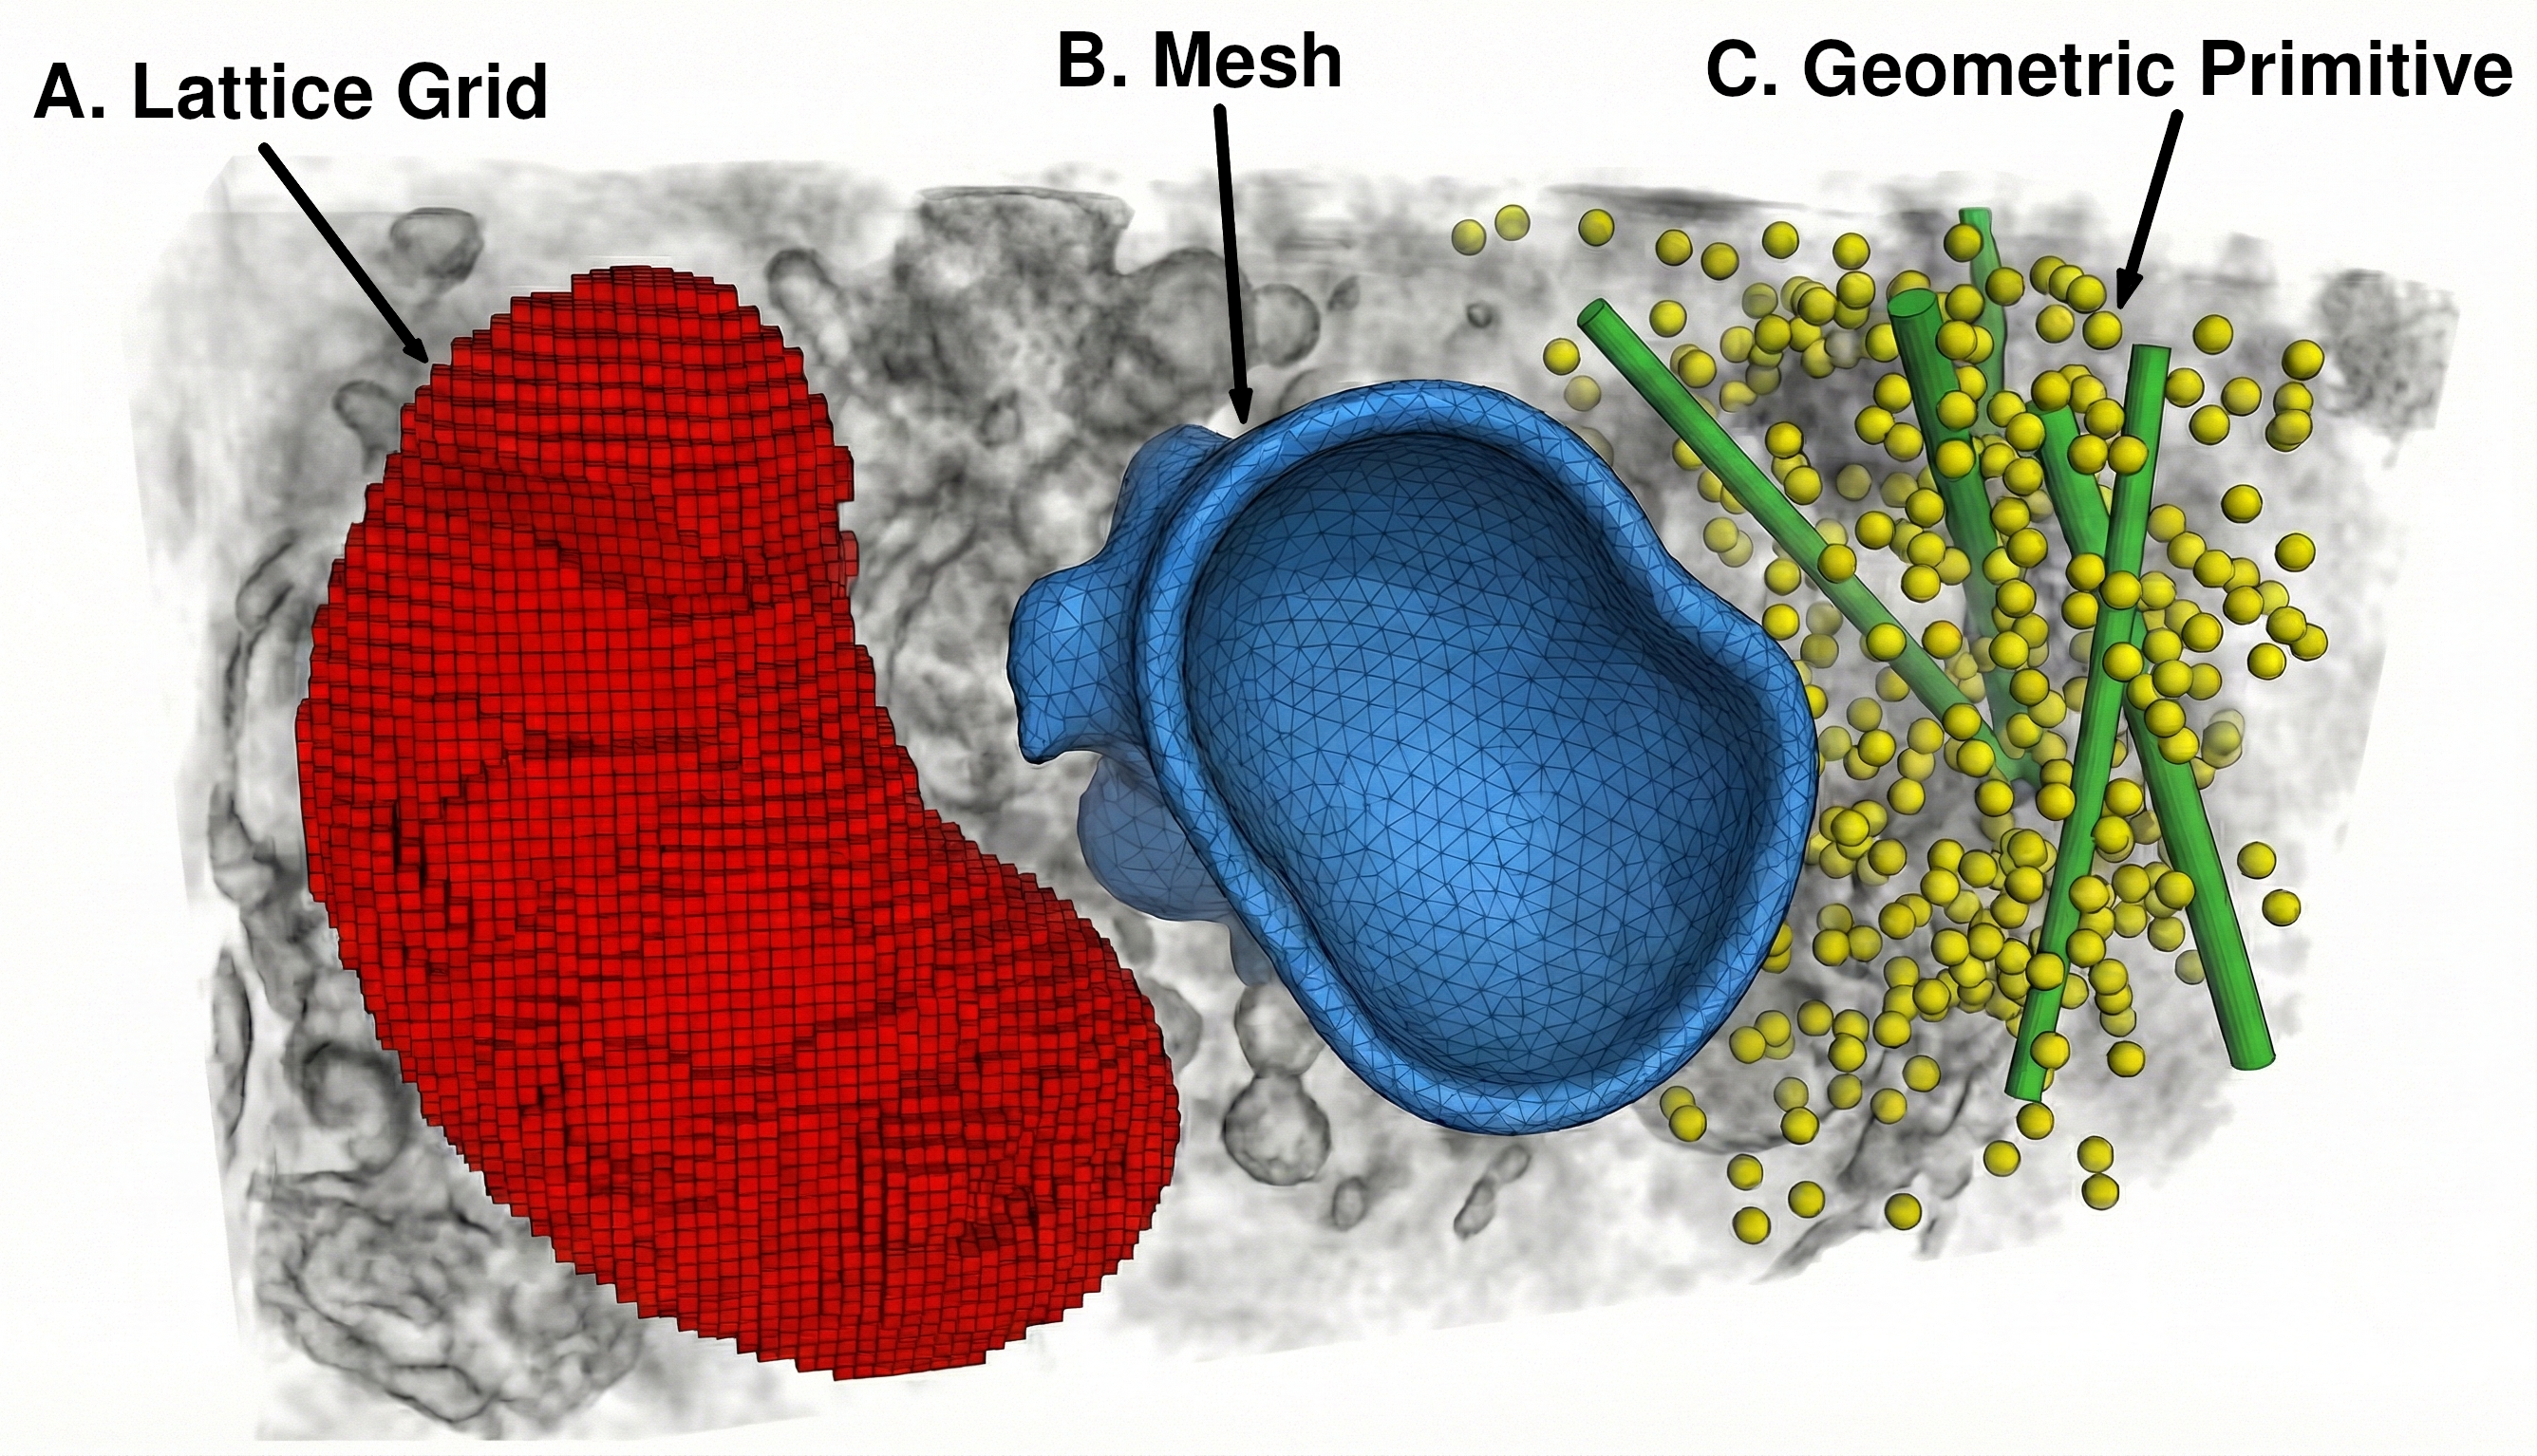
\includegraphics[width=0.8\textwidth]{images/segmentation-comparison.png}
    \caption[Comparison of segmentation representations]{Comparison of segmentation representations. (A) Lattice Grid: The structure is defined by a set of discrete voxels. (B) Mesh: The structure boundary is approximated by triangular faces. (C) Geometric Primitive: The structure is approximated by mathematical shapes (spheres and cylinders).}
    \label{figure:segmentation-comparison}
\end{figure}

\section{Semantic and Visual Annotations}
\label{section:annotations}

While segmentation provides the geometric boundaries of biological structures, it is the process of \textit{annotation} that assigns semantic meaning to these geometries. Without annotation, a segmented mesh is merely a generic shape; with annotation, it becomes an identified biological entity (e.g., ``ATP Synthase Complex'').

In the context of this thesis, we define annotations as the metadata and styling parameters that accompany raw volumetric and segmentation data. Unlike the structural data, which is objective and measured, annotations are subjective and interpretive, as shown in Figure~\ref{figure:annotations-explainer}. We categorize them into two functional groups:

\subsection{Descriptive Annotations}

Descriptive annotations provide semantic context. They link spatial regions to biological identities. Examples include:

\begin{itemize}
    \item \textbf{Labels:} Human-readable names (e.g., ``Outer Membrane'').
    \item \textbf{Descriptions:} Free-text scientific explanations or educational notes.
    \item \textbf{External References:} Database identifiers (e.g., Gene Ontology \cite{Consortium2023GO}, PDB \cite{Berman2000PDB}) that link the visual object to external knowledge bases.
\end{itemize}

\subsection{Visual Annotations}

Visual annotations dictate how the data is rendered to convey information effectively. In complex 3D scenes, visual properties are not merely aesthetic; they are also functional---they guide the viewer's attention. Examples include:

\begin{itemize}
    \item \textbf{Coloring:} assigning distinct colors to different biological components (e.g., DNA = blue, Histones = yellow).
    \item \textbf{Opacity/Transparency:} Adjusting alpha values to reveal internal structures (e.g., making a cell membrane semi-transparent to show organelles inside).
    \item \textbf{Thresholding:} Defining the specific isovalue level at which a volume should be rendered.
\end{itemize}

\begin{figure}[htbp]
    \centering
    \includegraphics[width=0.8\textwidth]{images/annotations-explainer.png}
    \caption[Impact of annotations on visualization]{(A) Geometric Representation: The structure is merely a geometric shape lacking context. (B) Annotated Scene: The application of visual annotations (coloring by chain ID) and descriptive annotations (text labels) transforms the geometry into an interpretable biological model.}
    \label{figure:annotations-explainer}
\end{figure}

\section{Volumetric Rendering Techniques}
\label{section:rendering}

Rendering three-dimensional scalar fields requires specialized techniques to project volumetric information onto a two-dimensional screen. There are three primary approaches employed in modern visualization software, as shown in Figure~\ref{figure:rendering}. Each of these approaches provides distinct tradeoffs between performance and information density.

\subsection{Direct Volume Rendering}

Direct volume rendering (DVR) visualizes the dataset as a semi-transparent cloud. It typically employs ray-marching algorithms, where ``rays'' are cast from the camera through the volume. As a ray traverses the grid, it samples density values at discrete steps, mapping them to color and opacity via a transfer function \cite{hansen2011visualisation}.

While visually rich, DVR is computationally expensive and requires significant graphics processing power.

\subsection{Isosurface Extraction}

An isosurface represents a three-dimensional boundary connecting all points in the volume that share a specific intensity value (the isovalue). This method effectively extracts a ``shell'' from the continuous data. Computationally, this reduces the volumetric array to a set of polygonal meshes (typically via Marching Cubes)  \cite{hansen2011visualisation}. 

This transformation allows for highly efficient rendering using standard graphics pipelines. The primary limitation is information loss: density variations inside or outside the chosen isosurface are completely discarded.

\subsection{Orthogonal Slices}

Slice visualization renders a single 2D plane cutting through the 3D volume, typically aligned with the principal axes ($xy$, $xz$, $yz$). While it lacks 3D spatial context, this method provides the most accurate view of the raw data \cite{hansen2011visualisation}. Unlike DVR or isosurfaces, which rely on accumulation or interpolation, slice views allow researchers to inspect the exact intensity values of individual voxels, making it essential for quality control and detailed analysis.

\begin{figure}[htbp]
    \centering
    \includegraphics[width=0.8\textwidth]{images/rendering.png}
    \caption[Volumetric rendering techniques]{(A) Direct Volume Rendering: Shows the internal structure using transparency. (B) Isosurface Extraction: Extracts a solid shell at a specific threshold, offering high performance at the cost of hiding internal details. (C) Orthogonal Slice: Displays raw voxel intensities along a 2D plane.}
    \label{figure:rendering}
\end{figure}

\section{State of the Art in Visualization Software}
\label{section:existing-visualisers}

The shift towards cloud-based data storage has driven the development of web-native visualization tools capable of streaming large volumetric datasets. While several robust solutions exist, they generally prioritize different domains than structural biology.

\subsection{Neuroglancer}

Neuroglancer \cite{shepard2021neuroglancer} is a viewer designed for navigating petabyte-scale datasets, particularly in the field of connectomics. It excels at handling multi-resolution data structures (pyramids) and slicing of massive volumes in arbitrary ways.

\textbf{Limitation:} Its user interface is highly technical, relying heavily on JavaScript Object Notation (JSON) state manipulation. Furthermore, it lacks native support for standard structural biology formats (like atomic models) and the simplified annotation tools required for educational or general research presentation.

\subsection{Vizarr}

Vizarr is a lightweight, modular viewer component explicitly designed for OME-NGFF images (both described in \cite{moore2021ome}). Its primary strength is modularity; it is designed to be embedded into other analysis platforms (like Napari or Jupyter) rather than serving as a standalone presentation tool.

\textbf{Limitation:} While excellent for raw image inspection, Vizarr does not provide the scene composition features—such as segmentation overlay—necessary for high-fidelity structural visualization.

\subsection{WebKnossos}
WebKnossos \cite{boergens2017webknossos} is a web-based platform optimized for the collaborative annotation of massive 3D electron microscopy datasets. It is particularly widely used in connectomics for skeletonizing neurons and segmenting complex tissue blocks.

\textbf{Limitation:} Similar to Neuroglancer, WebKnossos is specialized for data reconstruction and tracing tasks in neurobiology. It is not designed for structural biology applications that require superimposing atomic coordinates onto density maps or creating curated, stylized visualizations for publication.

\subsection{Napari}

Napari \cite{sofroniew2025napari} is a fast, interactive, multi-dimensional image viewer for Python. It has become a cornerstone of the bioimage analysis community due to its plugin ecosystem and ability to handle massive datasets seamlessly.

\textbf{Limitation:} Napari is primarily a desktop application designed for Python developers and data analysts. While web-based ports exist, they lack the stability of the core desktop application. Furthermore, its focus is on quantitative analysis and segmentation generation rather than the declarative ``presentation'' of completed biological stories.

\subsection{UCSF ChimeraX}

While primarily a desktop application, ChimeraX \cite{Meng2023ChimeraX} is a widely adopted tool for volumetric visualization in structural biology, offering high-quality rendering and extensive annotation capabilities.

\textbf{Limitation:} As a desktop application, it requires local installation and high-end hardware. It does not address the problem of ``zero-install'' accessibility and lightweight web sharing, which is the primary objective of this thesis.

\begin{sidewaystable}[p]
    \centering
    \caption[Comparison of visualization tools]{Comparison of existing visualization tools against the requirements of this thesis.}
    \label{tab:software-comparison}
    \begin{tabularx}{\textwidth}{l >{\hsize=0.6\hsize}X >{\hsize=0.6\hsize}X >{\hsize=1.8\hsize}X}
        \toprule
        \textbf{Software} & \textbf{Domain} & \textbf{Platform} & \textbf{Key Limitation for this Work} \\
        \midrule
        \textbf{Neuroglancer} & Connectomics & Web & Complex UI; lack of atomic model support. \\
        \addlinespace
        \textbf{Vizarr} & Image Analysis & Web Component & Lacks 3D scene composition tools. \\
        \addlinespace
        \textbf{WebKnossos} & EM Annotation & Web & Optimized for tracing, not structural presentation. \\
        \addlinespace
        \textbf{Napari} & Image Analysis & Desktop & Requires local installation/Python environment. \\
        \addlinespace
        \textbf{ChimeraX} & Structural Biology & Desktop & Not web-accessible; heavy resource requirements. \\
        \midrule
        \textbf{Mol* (Target)} & Structural Biology & Web & \textit{Base for the proposed solution.} \\
        \bottomrule
    \end{tabularx}
\end{sidewaystable}

For a comprehensive comparison of these tools, refer to Table~\ref{tab:software-comparison}.

In summary, while powerful tools exist for specific niches (e.g., connectomics, raw image analysis, and desktop rendering), there is a lack of a unified web-based solution that combines lightweight volumetric streaming with rich biological annotation. The Mol* ecosystem, introduced in the next chapter, provides the necessary foundation to bridge this gap.

\clearpage
\newpage
\chapter{Overview of the Mol* Ecosystem}
\label{chapter:molstar}

The practical contributions of this thesis are built upon the Mol* ecosystem, a state-of-the-art suite of tools for the visualization and analysis of macromolecular data. This chapter provides an overview of the core Mol* framework, the specific extension for volumetric data (Mol* Volumes and Segmentations), and the emerging MolViewSpec standard and MolViewStories application.

\section{Mol*}

Mol* (pronounced ``molstar'') is an open-source web-based toolkit designed for the visualization and analysis of large-scale biological data \cite{Sehnal2021Molstar}. 

Mol* provides a 3D viewer which contains a rich set of tools for manipulating the molecular scene, including representation and coloring schemes, component selection, and distance and angle measurements. Its utility is further enhanced by deep integration with major public databases as it serves as the primary 3D viewer for, among many others, the Protein Data Bank in Europe (PDBe) \cite{Armstrong2019pdbe}, the RCSB Protein Data Bank \cite{Berman2000PDB}, and AlphaFold DB \cite{Fleming2025alphafolddb}.

The architecture of Mol* is highly modular and contains an extension system that allows developers to create custom behavior that augments the core functionality without modifying the base code. This extensibility has led to the development of various specialized visualization tools, such as the Mol* Volumes and Segmentations \cite{Chareshneu2023Volseg}, the specific extension for microscopy data discussed in Section~\ref{section:volseg}.

\section{The mmCIF and BinaryCIF Formats} 
\label{section:binarycif}

The Mol* ecosystem relies heavily on the macromolecular Crystallographic Information File (mmCIF) \cite{Westbrook2022mmCIF} standard and its binary counterpart, BinaryCIF \cite{Sehnal2020BinaryCIF}, to handle complex structural and annotation data.

\subsection{The PDBx/mmCIF Standard}

Historically, the Protein Data Bank (PDB) \cite{Berman2000PDB} file format was the standard for structural biology. However, its fixed-column width architecture imposed significant limitations, such as a maximum of 99,999 atoms, which became obsolete with the determination of large macromolecular assemblies, initially by X-ray crystallography and increasingly by Cryo-EM. To address these limitations, the PDBx/mmCIF format was adopted as the official standard by the Worldwide Protein Data Bank (wwPDB) \cite{Westbrook2022mmCIF}.

The mmCIF format is a dictionary-based, key-value format. It organizes data into ``categories'' (tables) and ``items'' (columns), similar to a relational database schema. This flexibility allows mmCIF to store not only atomic coordinates but also extensive metadata, experimental details, and custom annotations.

\subsection{BinaryCIF}

While mmCIF solves the issue of extensibility, it remains a text-based format. This causes it to have an inherently large size, and it is inefficient to parse, particularly for the large density maps associated with electron tomography.

To overcome this bottleneck, the BinaryCIF format was developed as an efficient binary serialization of the CIF standard. BinaryCIF employs several encoding strategies, such as run-length encoding and integer packing, to minimize file size and maximize parsing 
speed \cite{Sehnal2020BinaryCIF}.

\section{Mol* Volumes and Segmentations}
\label{section:volseg}

Mol* Volumes and Segmentations (Mol* VS) \cite{Chareshneu2023Volseg} is a specialized Mol* extension designed to enable the visualization of 3D volumetric data, segmentations, and their associated biological annotations. It was developed to address the specific challenges of interpreting cellular imaging data found in public repositories such as EMDB \cite{wwPDBConsortium2023EMDB}, EMPIAR \cite{wwPDBConsortium2022EMPIAR}, BioImage Archive \cite{Hartley2022BioImageArchive}, and Image Data Resource (IDR) \cite{Williams2017IDR}.

By extending the scope of Mol* to the cellular scale, Mol* VS allows researchers to visualize organelles and macromolecular complexes within their native spatial context.

\subsection{Component Architecture}
\label{section:molstar-volseg-architecture}

The Mol* VS extension is highly modular and composed of five major components---Preprocessor, Database, Server, Client, and VSToolkit---the interaction of which is displayed in Figure~\ref{figure:volseg-arch}.

\begin{figure}[htbp]
    \centering
    \includegraphics[width=0.8\textwidth]{images/volseg-arch.pdf}
    \caption[Architecture of Mol* VS]{The architecture of Mol* VS, illustrating the data flow from raw input files through the preprocessor, database, and server to the client and the VSToolkit. Image redrawn from \cite{Chareshneu2023Volseg}.}
    \label{figure:volseg-arch}
\end{figure}

\subsubsection{Preprocessor}

The entry point of the pipeline. It accepts volumetric and segmentation data in various file formats. The preprocessor converts these inputs into the OME-NGFF format. Crucially, it performs downsampling of the processed data, which allows streaming large datasets by serving lower-resolution data.

\subsubsection{Database}

A storage layer that houses the preprocessed OME-NGFF data. Can hold multiple downsampled versions of the data.

\subsubsection{Server}

An HTTP server responsible for querying the database. It handles requests from the client, fetching specific data (volumes, segmentations, metadata) and streaming them to the browser.

\subsubsection{Client}

A Mol* extension that renders the data in the Mol* Viewer and allows users to control visual parameters such as color, opacity, and isosurface levels, as well as interact with annotations---displaying and editing.

\subsubsection{VSToolkit}

A standalone command-line tool designed for local data management. It allows users to query, package, and compress volumetric and segmentation data into an archive file known as CVSX. This component acts as a container encapsulating all metadata and raw data files necessary to load into the Mol* Viewer. This effectively bypasses the need for a dedicated server infrastructure, enabling data portability and sharing.

\subsection{CVSX File Format}
\label{subsection:cvsx-file-format}

The Cell* Volumes \& Segmentations Archive (CVSX) format was introduced with the VSToolkit to allow users to share the visualization sessions without relying on the server component \cite{Chareshneu2024Volseg}. 

Technically, a CVSX file is a ZIP archive containing a specific directory structure that encapsulates all volume and segmentation files, as well as the biological annotations and the metadata required to render the scene.

The internal structure of a CVSX file comprises:

\begin{itemize}
    \item \textbf{Index:} A JSON file which describes the contents of the ZIP archive.
    \item \textbf{Metadata:} JSON file that defines the information about the volume and segmentation data, such as the dimensions of the volume and the available downsampling levels.
    \item \textbf{Annotations:} A JSON structure mapping the volumetric and segmentation entries to human-readable descriptions, colors, and external database references.
    \item \textbf{Query:} A JSON file describing the exact parameters used to query the data from the database.
    \item \textbf{Structural Data:} The actual binary data for the volume and segmentations (lattices, meshes, or geometric), stored in the BinaryCIF format (geometric segmentations are stored in JSON files).
\end{itemize}

\subsection{Limitations of the Current Approach}
\label{section:volseg-limitations}

Despite the utility of Mol* VS and the CVSX format, several limitations have emerged that necessitate a modernized approach:

\begin{enumerate}
    \item \textbf{Maintenance and Deprecation:} The development of the Mol* VS Client component has stagnated, and it is no longer actively maintained. As the core Mol* Viewer evolves, the legacy Mol* VS extension becomes increasingly prone to compatibility issues and bugs.
    
    \item \textbf{Rigid Annotation Capabilities:} The annotation system within CVSX is limited. While it supports basic labels and descriptions, it lacks the ability to create narrative flows or guide the user through specific viewpoints (e.g., ``stories''). This stands in stark contrast to modern storytelling tools like MolViewStories, which allow researchers to craft guided interactive experiences. Furthermore, the mechanisms for editing these annotations in the legacy client are user-unfriendly. Although the Mol* VS Client includes a built-in annotation editor, it provides only a raw JSON view and, critically, lacks the capability to save changes back to local CVSX files---it is restricted to updating server-hosted entries. Therefore, modifying a portable CVSX archive necessitates manual JSON manipulation and file re-packaging using the VSToolkit CLI, presenting a high barrier to entry for non-technical users.
    
    \item \textbf{Isolation from the Ecosystem:} Data stored in CVSX is effectively siloed. It is challenging to compose a scene that combines a CVSX volume with other data types supported by Mol* (such as atomic models from the PDB archive) without complex custom coding. The viewer state is tightly coupled to the specific logic of the Mol* VS extension rather than a standard scene description.
\end{enumerate}

\section{MolViewSpec}
\label{section:molviewspec}

The most significant recent advancement in the Mol* ecosystem is the introduction of the MolViewSpec (MVS) \cite{Midlik2025MolViewSpec}---a declarative, platform-independent standard for describing molecular visualizations.

Historically, reproducing a specific visual state across different software platforms has been a persistent challenge in structural biology \cite{Midlik2025MolViewSpec}. The traditional approaches can be categorized into three distinct methods, each with significant limitations:

\begin{itemize}
    \item \textbf{Interactive Sessions:} Saved state files (e.g., Mol* sessions) are binary ``black boxes'' that are difficult to edit programmatically and impossible to open in other software.
    \item \textbf{Imperative Scripts:} Scripting languages (e.g., ChimeraX command scripts) describe \textit{how} to achieve a result (step-by-step instructions). These are fragile; if the underlying data changes slightly, the script often breaks.
    \item \textbf{URL Parameters:} Web viewers often use URL parameters, but these are limited in length and expressiveness, unable to describe complex scenes with multiple superimposed structures.
\end{itemize}

MolViewSpec addresses these issues by adopting a declarative approach. Instead of listing the individual steps to create a scene, MVS describes the final hierarchy of the scene itself.

\subsection{The MVS Tree Structure (MVSJ)}
\label{section:mvsj-format}

At the core of the standard is the MolViewSpec JSON (MVSJ) format. The visualization state is represented as a hierarchical tree structure, as depicted in Figure~\ref{fig:mvs-comparison}.

\subsubsection{Tree Processing}

In a standard scene, the processing logic flows from the root of the tree downwards, typically following this hierarchy:

\begin{enumerate}
    \item \textbf{Data Retrieval:} The root branches define where to fetch data (e.g., \texttt{download} node fetching a file from a URL).
    \item \textbf{Parsing:} Children of data nodes define how to interpret the fetched data (e.g., \texttt{parse} node treating the data as mmCIF or BinaryCIF).
    \item \textbf{Structure Derivation:} These nodes extract the biological model from the parsed data (e.g., \texttt{structure} node selecting Model 1, Assembly 1).
    \item \textbf{Component Selection:} Specific parts of the structure are selected (e.g., \texttt{component} node selecting ``Polymer Chain A'' or ``Ligands'').
    \item \textbf{Visual Representation:} Visual representations are applied to the selected components (e.g., ``Render as Cartoon, Color: Blue''). 
\end{enumerate}

\begin{figure}[htbp]
    \centering

    \begin{subfigure}{\textwidth}
        \centering
        \includegraphics[height=0.45\textheight]{images/mvs-tree-example.pdf}
        \caption{MVS tree representation.}
        \label{fig:mvs-tree}
    \end{subfigure}

    \vspace{1em}

    \begin{subfigure}{\textwidth}
        \centering
        \includegraphics[height=0.30\textheight]{images/1CBS.png}
        \caption{Rendered visual output.}
        \label{fig:mvs-output}
    \end{subfigure}

    \caption[MVS tree and output comparison]{Comparison between the MVS tree representation (\subref{fig:mvs-tree}) 
and its corresponding rendered visual output (\subref{fig:mvs-output}).}
    \label{fig:mvs-comparison}
\end{figure}

\subsubsection{MVSJ Modes}

The MVSJ format supports two structural modes:

\begin{itemize}
    \item \textbf{Single Mode:} The tree defines a ``single'' root node. This configuration represents a single, standalone visualization scene.
    \item \textbf{Multiple Mode:} The structure contains a ``multiple'' node which acts as a container for several distinct root nodes. This allows a single MVSJ file to encapsulate multiple independent visual states or ``stories''. This mode will be referred to as MVS stories.
\end{itemize}

\subsection{MVS Stories}
\label{section:mvs-stories}

While the single-mode MVSJ tree defines a single static snapshot of a scene, MVS stories introduce the concept of temporal progression and narrative.

An MVS story is composed of a sequence of MVS snapshots, or ``slides''---each containing a MVSJ tree and metadata (title, description). Users can navigate through these slides to view different aspects of the data, accompanied by descriptive text and annotations. This tool is particularly valuable for educational purposes and scientific communication, as it allows authors to guide the viewer's attention through complex structural features step-by-step \cite{Midlik2025MolViewSpec}.

\subsection{The MVSX File Format}
\label{section:mvsx-format}

While MVSJ provides the instructions for building a scene, it typically relies on external URLs to retrieve data. To solve the issue of portability, the MVSX archive format was introduced.

MVSX is a ZIP archive that packages the MVSJ state file together with all referenced data files (e.g., mmCIF models, BinaryCIF volumes) into a single container. Relative paths are used within the MVSJ tree to point to the files inside the archive. This ensures that the visualization is self-contained and reproducible, even in offline environments.

\subsection{Builder Libraries}

To facilitate the generation of these MVSJ trees, the authors provide official builder libraries in both Python\footnote{\url{https://github.com/molstar/mol-view-spec}} and TypeScript\footnote{\url{https://github.com/molstar/molstar}}. These libraries provide a type-safe builder pattern that allows developers to construct the scene graph programmatically.

\subsection{MolViewStories}
\label{section:molviewstories}

MolViewStories\footnote{\url{https://molstar.org/mol-view-stories}} is a web application that combines the advanced 3D rendering capabilities of Mol* with a story-building interface based on the MolViewSpec standard. Unlike traditional point-and-click viewers, it features a code-driven scene builder---essentially a built-in TypeScript editor that provides direct access to the MolViewSpec API. This allows users to programmatically define molecular scenes, representations, and animations with immediate visual feedback, as shown in Figure~\ref{fig:molviewstories}.

The application allows researchers to combine individual scenes into cohesive interactive stories, complete with narrative descriptions and smooth transitions. Furthermore, it addresses the data portability issues of previous generations by offering native cloud storage and sharing capabilities, enabling visualizations to be published and accessed via persistent URLs.

\begin{figure}[htbp]
    \centering
    \includegraphics[width=0.8\textwidth]{images/molviewstories.png}
    \caption[The MolViewStories interface]{The MolViewStories interface. The left panel contains the TypeScript editor for defining scene states using the MVS builder library, while the right panel provides real-time visual feedback through the Mol* Viewer.}
    \label{fig:molviewstories}
\end{figure}

\subsection{The MVStory Format}
\label{section:mvstory-format}

The MolViewStories application persists its state in a custom archive format. While the MVSJ tree describes a single static scene, the MVStory format encapsulates an entire interactive narrative, describing a collection of scenes, the transitions between them, and the assets required to render them.

Technically, the format is a MessagePack serialized binary file, typically compressed within a ZIP container. The internal structure is defined by the \texttt{StoryContainer} root object, which holds the versioning information and the main \texttt{Story} object. The complete data model is visualized in Figure~\ref{fig:mvstory-data-model}.

\begin{figure}[htbp]
    \centering
    \includegraphics[width=0.8\textwidth]{images/mvstory.pdf}
    \caption[MVStory data model]{Class diagram representing the internal structure of the MVStory format.}
    \label{fig:mvstory-data-model}
\end{figure}

\part{Practical Contributions}

\clearpage
\newpage
\chapter{Conversion Library}
\label{chapter:library}

To bridge the gap between the legacy CVSX format and the modern MolViewSpec standard, we developed a Python conversion library. This chapter details the engineering principles behind the library. Section~\ref{sec:library-requirements} outlines the functional requirements. Section~\ref{sec:architecture-and-design} describes the architectural patterns, data mapping strategies, and data models employed. Section~\ref{section:library-implementation} details the algorithmic implementation of the transformation logic, and finally Section~\ref{section:library:results} discusses the verification of the results.

\section{Requirements}
\label{sec:library-requirements}

The specific requirements for the conversion library are as follows:

\begin{enumerate}
    \item \textbf{Visual Fidelity:} The visual representation in the Mol* Viewer must match the original CVSX entry visualization as closely as possible within the constraints of the MVS standard.
    
    \item \textbf{Data Integrity:} The underlying volumetric data, segmentations, and annotations must be preserved without data loss.
    
    \item \textbf{Memory Efficiency:} The library must handle large volumetric datasets efficiently.
\end{enumerate}

\section{Architecture and Design}
\label{sec:architecture-and-design}

Converting the CVSX format involves processing multiple heterogeneous file formats. A simple imperative script would quickly become unmanageable and difficult to test. Therefore, the library is designed with a strict architectural framework in mind to prioritize modularity and separation of concerns.

\subsection{Pipeline Architecture}
\label{subsection:pipeline-architecture}

To manage the complexity of the data flow, the library adopts a multi-stage pipeline architecture. While conceptually similar to the Extract-Transform-Load (ETL)\footnote{\url{https://learn.microsoft.com/en-us/azure/architecture/data-guide/relational-data/etl}} pattern used in data warehousing, this implementation adapts the concept for file conversion.

The ETL process is divided into three distinct stages:

\begin{enumerate}
    \item \textbf{Extract:} Responsibilities include validating the input CVSX archive and abstracting access to the volumetric and segmentation files within it.
    
    \item \textbf{Transform:} This is the core of the library. It converts the format-specific input into an intermediate representation. It handles geometric calculations, such as generating meshes from lattice data.
    
    \item \textbf{Load:} The final stage consumes the intermediate representation and serializes it into the specific target format (MVSX or MVStory).
\end{enumerate}

The detailed pipeline is depicted in Figure~\ref{figure:etl-pipeline}.

\begin{figure}[htbp]
    \centering
    \includegraphics[height=0.9\textheight]{images/etl-pipeline.pdf}
    \caption[ETL pipeline architecture]{The ETL pipeline architecture adopted by the library.}
    \label{figure:etl-pipeline}
\end{figure}

\subsection{Data Mapping Strategy}
\label{subsection:data-mapping}

A critical design challenge was mapping the heterogeneous data types found in CVSX to the MVS tree hierarchy. Figure~\ref{fig:mapping-complete-flow} illustrates how the library implements specific transformation logic for each data type.

\begin{figure}[htbp]
    \centering
    \includegraphics[width=1\textwidth]{images/mapping.pdf}
    \caption[CVSX-MVS data mapping flow]{CVSX-MVS data mapping flow.}
    \label{fig:mapping-complete-flow}
\end{figure}

\subsubsection{Volume Classification}
In the CVSX format, all density data is stored as 3D arrays. However, functionally, some of these arrays represent 3D isosurfaces while others represent single 2D slices. For this reason, the library implements a classification step that inspects the dimensionality of the input volume. If any dimension has a size of 1 (e.g., $1 \times 512 \times 512$), it is mapped to the MVS \texttt{Grid Slice} volume representation; otherwise, it is mapped to the MVS \texttt{Isosurface} volume representation.

\subsubsection{Lattice Segmentation Pipelines}

Lattice segmentations (integer voxel masks) present a unique challenge as they can be represented in MVS in two distinct ways---either as volumes or as surface meshes. The design supports both approaches:

\begin{itemize}
    \item \textbf{Lattice-to-Volume:} Preserves the volumetric nature of the data. It isolates specific segments via binary masking and re-encodes them as independent volumes.

    \item \textbf{Lattice-to-Mesh:} Converts the voxel data into surface meshes using the Marching Cubes algorithm.
\end{itemize}

\subsubsection{Geometric Transformation}
Geometric segmentations in CVSX are defined mathematically (e.g., spheres are defined by a center point and radius). The design categorizes these shapes into two groups based on MVS support:
\begin{itemize}
    \item \textbf{Direct Mapping:} Shapes supported natively by MVS (spheres, boxes, ellipsoids, and uniform cylinders) are mapped directly.

    \item \textbf{Procedural Generation:} Shapes without direct MVS counterparts (pyramids and tapered cylinders) are transformed into meshes and mapped to the MVS mesh primitive node.
\end{itemize}

\subsection{Data Models}
\label{subsection:data-models}

To support the conversion pipeline, four distinct data models were designed. These models structure the data at various stages of the conversion process and enforce strict typing to prevent working with malformed data.

\subsubsection{CVSX Model (Input)}

The CVSX Model mirrors the schema of the legacy file format detailed in Section~\ref{subsection:cvsx-file-format}. It contains the deserialized JSON files---Index, Annotations, Metadata, and Query---and a list of pointer objects to the raw data files. Crucially, this model implements a lazy-loading mechanism. The binary data is not read during the initialization of the CVSX Model; instead, it is accessed on-demand via the file proxy system described in Section~\ref{section:optimizing}.

\subsubsection{Internal Model}
\label{subsection:internal-model}

The \texttt{InternalEntry} model serves as the intermediate representation. It abstracts away the idiosyncrasies of the file system inside the CVSX zip archive and specific file formats. As shown in Figure~\ref{figure:internal}, it groups the data hierarchically by timeframe. It references all transformed volumetric and segmentation objects, providing a unified structure that is independent of the input source.

\begin{figure}[htbp]
    \centering
    \includegraphics[width=0.8\textwidth]{images/internal.pdf}
    \caption[Internal model]{Internal model used by the conversion library as an intermediate model in the transform phase.}
    \label{figure:internal}
\end{figure}

\subsubsection{MVSX and MVStory Models (Output)}

These models represent the corresponding output file formats and are created from the internal model through their respective transformers.

\begin{itemize}
    \item The \texttt{MVSXEntry} model contains a list of MVS stories and a directory of assets to which the nodes point using relative paths.
    
    \item The \texttt{MVStoryEntry} model wraps the StoryContainer model (Figure~\ref{fig:mvstory-data-model}).
\end{itemize}

\section{Implementation}
\label{section:library-implementation}

This section details the specific implementation strategies used to meet the requirements.

\subsection{Used Technologies}

The conversion library is implemented in Python, which was primarily chosen for the availability of the MolViewSpec library.

The implementation relies on a set of core dependencies, each selected to handle specific aspects of the conversion pipeline:

\begin{itemize}
    \item \textbf{MolViewSpec\footnote{\url{https://pypi.org/project/molviewspec}}:} Used to programmatically construct the MVS nodes.
    
    \item \textbf{Pydantic\footnote{\url{https://pypi.org/project/pydantic}}:} Used for schema definition and data validation. Ensures that any schema mismatches are caught early in the pipeline.
    
    \item \textbf{NumPy\footnote{\url{https://pypi.org/project/numpy}}:} Used for handling the large 3D voxel arrays associated with volumetric data and for performing linear algebra operations required for the transformations.
    
    \item \textbf{CIFTools\footnote{\url{https://pypi.org/project/ciftools}}:} A library for parsing and writing BinaryCIF files. It is used for reading the raw volume, lattice segmentation, and mesh segmentation data from the CVSX archive and serializing the result of the converted lattice segmentations.
    
    \item \textbf{Scikit-image\footnote{\url{https://pypi.org/project/scikit-image}}:} Provides the implementation of the Marching Cubes algorithm used for isosurface extraction.
    
    \item \textbf{Msgpack\footnote{\url{https://pypi.org/project/msgpack}}:} Used for the binary serialization of the MVStory format.
\end{itemize}

\subsection{Optimizing Memory with Lazy Loading}
\label{section:optimizing}

A critical requirement was the ability to handle large datasets efficiently. To achieve this, the implementation utilizes a proxy pattern via a \texttt{FileProxy} class.

When a CVSX archive is opened, the library parses the index and metadata JSON files immediately, but it does not read the binary files containing volumes or segmentations. Instead, it instantiates \texttt{FileProxy} objects as depicted in Figure~\ref{figure:file-proxies}. These objects encapsulate the file path and the specific parsing logic required for that file type. The heavy binary data is loaded into memory only at the exact moment it is required by the transformer.

\begin{figure}[htbp]
    \centering
    \includegraphics[width=0.8\textwidth]{images/file-proxies.pdf}
    \caption[File proxy model]{File proxy model is used for lazy loading of large files in the pipeline.}
    \label{figure:file-proxies}
\end{figure}

\subsection{Lattice Segmentation Processing}
\label{section:impl-lattice}

The conversion of lattice segmentations (voxel masks) into surface meshes represents the most computationally intensive part of the library. The \texttt{LatticeTransformer} implements a multi-step pipeline to ensure the resulting meshes are as visually similar as possible to the original CVSX.

To optimize processing time, the implementation utilizes the \texttt{find\allowbreak\_objects} algorithm. Instead of processing the entire $N \times M \times D$ volume for every segment ID—which would be prohibitively slow for segmentations with hundreds of biological components—the algorithm calculates the bounding box for each unique segment ID. The generic Marching Cubes algorithm is then run only on this cropped sub-volume.

The pipeline for a single lattice segment proceeds as follows:
\begin{enumerate}
    \item \textbf{Extraction:} The specific integer ID is isolated from the volume.
    
    \item \textbf{Padding:} The sub-volume is padded with a 1-voxel border of zeros. This ensures that the generated mesh is closed and does not have ``holes'' where the structure touches the grid boundary.
    
    \item \textbf{Smoothing:} A smoothing kernel is applied to the binary mask to reduce the ``blocky'' artifacts typical of raw voxel data.
    
    \item \textbf{Meshing:} The Marching Cubes algorithm generates vertices and triangular faces.
    
    \item \textbf{Transformation:} The vertices, initially in local grid coordinates, are transformed into physical Angstrom coordinates using the voxel size and origin offset defined in the CVSX metadata. This is done so that the result mesh has an accurate size when loaded into the Mol* Viewer
\end{enumerate}

\subsection{Story Code Generation}

Unlike the MVSX format, which contains a single MVSJ file, the MVStory format is used in the MolViewStories application, where the MVS scene is built using the JavaScript library, as shown in Figure~\ref{fig:molviewstories}. 

The \texttt{StoriesTransformer}, therefore, functions as a code generator. It iterates through the internal model and uses string templates to construct valid JavaScript code. For every volume and segmentation, it generates a builder chain that downloads the data and applies the specific visual styling (color, opacity, tooltips) defined in the CVSX annotations.

This transformer is particularly significant for 4D datasets (time series). By iterating through the sequential timeframes of the internal model, the transformer automatically maps each timepoint to a distinct ``slide'' in the output story. This effectively linearizes the temporal dimension, generating a ready-made presentation where users can scrub through the biological process (e.g., a conformational change) frame-by-frame. This automatic scaffold saves the user from the tedious task of manually defining state transitions for every time point.

\subsection{Metadata Enrichment}
\label{section:fetching-isovalues}

For entries sourced from the EMDB repository, the library queries the public API of EMDB for author-recommended contour levels (isovalues). These isovalues are then injected into the internal model, ensuring that the resulting visualization of the volume corresponds to the experimentally determined density threshold.

\subsection{Availability}

The conversion library is available in the PyPI repository under the package name \texttt{cvsx2mvsx}\footnote{\url{https://pypi.org/project/cvsx2mvsx}}. Additionally, a Command Line Interface (CLI) is exposed via the \texttt{cvsx2mvsx} package's entry point for use in shell scripts. The CLI arguments are defined in Table~\ref{table:cli-arguments}.

\begin{table}[htbp]
    \centering
    \caption[CLI tool arguments]{The mvsx2cvsx CLI tool arguments.}
    \label{table:cli-arguments}
    \begin{tabularx}{\textwidth}{l X l}
        \toprule
        \textbf{Argument} & \textbf{Description} \\
        \midrule
        \texttt{-{}-input} & Path to the input \texttt{.cvsx} file.\\
        \texttt{-{}-output} & Path to the output file (\texttt{.mvsx} or \texttt{.mvstory}). \\
        \texttt{-{}-format} & Output format type (\texttt{mvsx} or \texttt{mvstory}).\\
        \texttt{-{}-lattice-to-mesh} & Use Marching Cubes conversion for lattice data. \\
        \bottomrule
    \end{tabularx}
\end{table}


\section{Verification and Results}
\label{section:library:results}

To validate the conversion library, we performed a comparison between the original CVSX visualizations (rendered in the legacy Mol* VS Client) and the converted MVSX visualizations (rendered in the modern Mol* Viewer). The verification process focused on three key metrics: visual fidelity, correctness of annotation handling, and storage efficiency.

\subsection{Dataset Selection}
\label{section:dataset-selection}

The robustness of the library was tested against a diverse dataset curated to cover the full spectrum of data types and edge cases present in the legacy VolSeg ecosystem. The test suite comprises 14 distinct datasets sourced from central biological archives, including EMDB, IDR, and EMPIAR.

The selected datasets were chosen to evaluate specific conversion challenges:

\begin{itemize}
    \item \textbf{Data Variety:} The set includes examples of all primary segmentation types: lattice grids (e.g., IDR-6001240), surface meshes (e.g., EMPIAR-10070), and geometric primitives (e.g., EMPIAR-11756).
    
    \item \textbf{Scale:} The data ranges from individual macromolecular structures or protein complexes occupying tens of kilobytes (e.g., EMD-1832) to large-scale quantitative cellular maps requiring hundreds of megabytes (e.g., IDR-5514375).

    \item \textbf{Composition:} We included entries with both single (e.g., EMPIAR\allowbreak-19111) and multiple timeframes (e.g., IDR-13457537), as well as entries combining density volumes with overlapping segmentation masks (e.g., EMD-1273).
\end{itemize}

A detailed overview of the selected datasets, including their sources, compositions, and file sizes, is presented in Table~\ref{tab:dataset-overview}.

\begin{table}[htbp]
    \centering
    \caption[Overview of selected datasets]{Detailed overview of the CVSX datasets used for verification. The table lists the dataset IDs with links to the source repositories, the image dimensions (XYZ = axes, C = channels, T = timeframes), the type and count of segmentations, and the original CVSX file size.}
    \label{tab:dataset-overview}
    \resizebox{\textwidth}{!}{
    \begin{tabular}{l r@{${}\times{}$}r@{${}\times{}$}r@{${}\times{}$}r@{${}\times{}$}l lrr}
        \toprule
        \textbf{Dataset ID} & \multicolumn{5}{c}{\textbf{Image dimensions (XYZCT)}} & \textbf{Seg. type} & \textbf{Seg. count} & \textbf{Size (MB)} \\
        \midrule
        \href{https://www.ebi.ac.uk/emdb/EMD-1832}{EMD-1832} & 64 & 64 & 64 & 1 & 1 & Lattice & 1 & 0.09 \\
        \href{https://www.ebi.ac.uk/emdb/EMD-1273}{EMD-1273} & 2048 & 2048 & 76 & 1 & 1 & Lattice & 5 & 39.78 \\
        \href{https://www.ebi.ac.uk/emdb/EMD-19111}{EMD-19111} & 440 & 440 & 440 & 1 & 1 & - & - & 12.15 \\
        \href{https://idr.openmicroscopy.org/webclient/img_detail/6001240}{IDR-6001240} & 271 & 275 & 236 & 2 & 1 & Lattice & 1 & 40.66 \\
        \href{https://idr.openmicroscopy.org/webclient/img_detail/6001247}{IDR-6001247} & 253 & 210 & 257 & 2 & 1 & Lattice & 1 & 35.43 \\
        \href{https://idr.openmicroscopy.org/webclient/img_detail/13457537}{IDR-13457537} & 198 & 223 & 12 & 6 & 18 & Lattice & 1 & 28.03 \\
        \href{https://idr.openmicroscopy.org/webclient/img_detail/5514375}{IDR-5514375} & 256 & 256 & 31 & 3 & 40 & Lattice & 2 & 493.08 \\
        \href{https://idr.openmicroscopy.org/webclient/img_detail/5025551}{IDR-5025551} & 2702 & 2700 & 1 & 18 & 1 & - & - & 65.92 \\
        \href{https://idr.openmicroscopy.org/webclient/img_detail/5025552}{IDR-5025552} & 2701 & 2701 & 64 & 18 & 1 & - & - & 63.29 \\
        \href{https://idr.openmicroscopy.org/webclient/img_detail/5025553}{IDR-5025553} & 2500 & 2500 & 64 & 21 & 1 & - & - & 96.63 \\
        \href{https://www.ebi.ac.uk/empiar/EMPIAR-10070}{EMPIAR-10070} & 1675 & 1595 & 291 & 1 & 1 & Mesh & 1 & 56.30 \\
        \href{https://www.ebi.ac.uk/empiar/EMPIAR-11756}{EMPIAR-11756} & 1024 & 1024 & 512 & 1 & 1 & Geometric & 1164 & 3.93 \\
        \href{https://cryoetdataportal.czscience.com/runs/17803}{CUSTOM-19420} & 1260 & 1260 & 368 & 1 & 1 & - & - & 32.22 \\
        \href{https://docs.openmicroscopy.org/ome-model/5.6.3/ome-tiff/data.html}{CUSTOM-TUBHISWT} & 512 & 512 & 10 & 2 & 43 & - & - & 106.10 \\
        \bottomrule
    \end{tabular}
    }
\end{table}

\subsection{Visual Fidelity}
\label{section:visual-fidelity}

We assessed the visual output across all supported data types. For the majority of datasets, the conversion produced visualizations that are structurally identical to the original. We analyzed six distinct visualization categories:

\begin{enumerate} 
    \item \textbf{Volume Isosurfaces:} The standard rendering for volumetric data. 
    \item \textbf{Volume Slices:} 2D slices of 3D data. 
    \item \textbf{Lattice Segmentation (Volume):} Voxel-based rendering of segmentation masks. 
    \item \textbf{Lattice Segmentation (Mesh):} Surface-based rendering derived from voxel masks. 
    \item \textbf{Mesh Segmentation:} Pre-calculated surface meshes. 
    \item \textbf{Geometric Segmentation:} Parametric shapes (spheres, cylinders, etc.). 
\end{enumerate}

In the case of Lattice-to-Mesh conversion (Figure~\ref{fig:emd-1832}), a slight visual difference is expected; the original volume representation appears smooth due to interpolation, whereas the converted mesh representation may appear slightly ``choppier'' depending on the resolution of the underlying grid and the Marching Cubes extraction. However, the spatial extent remains accurate.

\begin{figure}[htbp]
    \centering
    \begin{subfigure}{0.45\textwidth}
        \centering
        \includegraphics[width=\textwidth]{images/emd-1832-original.png}
        \caption{Legacy CVSX rendering.}
        \label{fig:emd-1832-mesh}
    \end{subfigure}
    \hfill
    \begin{subfigure}{0.45\textwidth}
        \centering
        \includegraphics[width=\textwidth]{images/emd-1832-mesh.png}
        \caption{MVSX rendering.}
        \label{fig:emd-1832-original}
    \end{subfigure}
    \caption[Lattice-to-Mesh representation]{Comparison of the original volume representation and the converted mesh representation of dataset EMD-1832.}
    \label{fig:emd-1832}
\end{figure}

\subsection{Correction of Legacy Artifacts}

During the verification process, we identified several instances where the legacy Mol* VS Client failed to render data correctly. In these cases, our conversion library not only preserved the data but also corrected the visualization errors inherent in the legacy software.

\subsubsection{Missing Volumes}

The original CVSX file for the EMD-1273 dataset contains a volume and five lattice segmentations. The legacy client fails to render the volume entirely, as shown in Figure~\ref{fig:volumes-problems}, due to an internal bug related to selecting an appropriate isovalue. The converted MVSX file successfully visualizes both the segmentations and the underlying volume.

\begin{figure}[htbp]
    \centering
    \begin{subfigure}{0.45\textwidth}
        \centering
        \includegraphics[width=\textwidth]{images/volume-missing.png}
        \caption{Legacy CVSX rendering.}
        \label{fig:volume-missing}
    \end{subfigure}
    \hfill
    \begin{subfigure}{0.45\textwidth}
        \centering
        \includegraphics[width=\textwidth]{images/volume-present.png}
        \caption{MVSX rendering.}
        \label{fig:volume-present}
    \end{subfigure}
    \caption[Correction of missing volumes]{Correction of missing volume for dataset EMD-1273.}
    \label{fig:volumes-problems}
\end{figure}

\subsubsection{Missing Annotations}

The IDR-6001240 dataset contains rich color annotations for both volumes and lattice segmentations. The legacy client fails to apply these colors, rendering the entire scene in a generic dark grey color, as shown in Figure~\ref{fig:visual-comparison}. The conversion library correctly parses the annotation JSON and applies the colors to the MVS tree, restoring the semantic meaning of the visualization.

\begin{figure}[htbp]
    \centering
    \begin{subfigure}{0.45\textwidth}
        \centering
        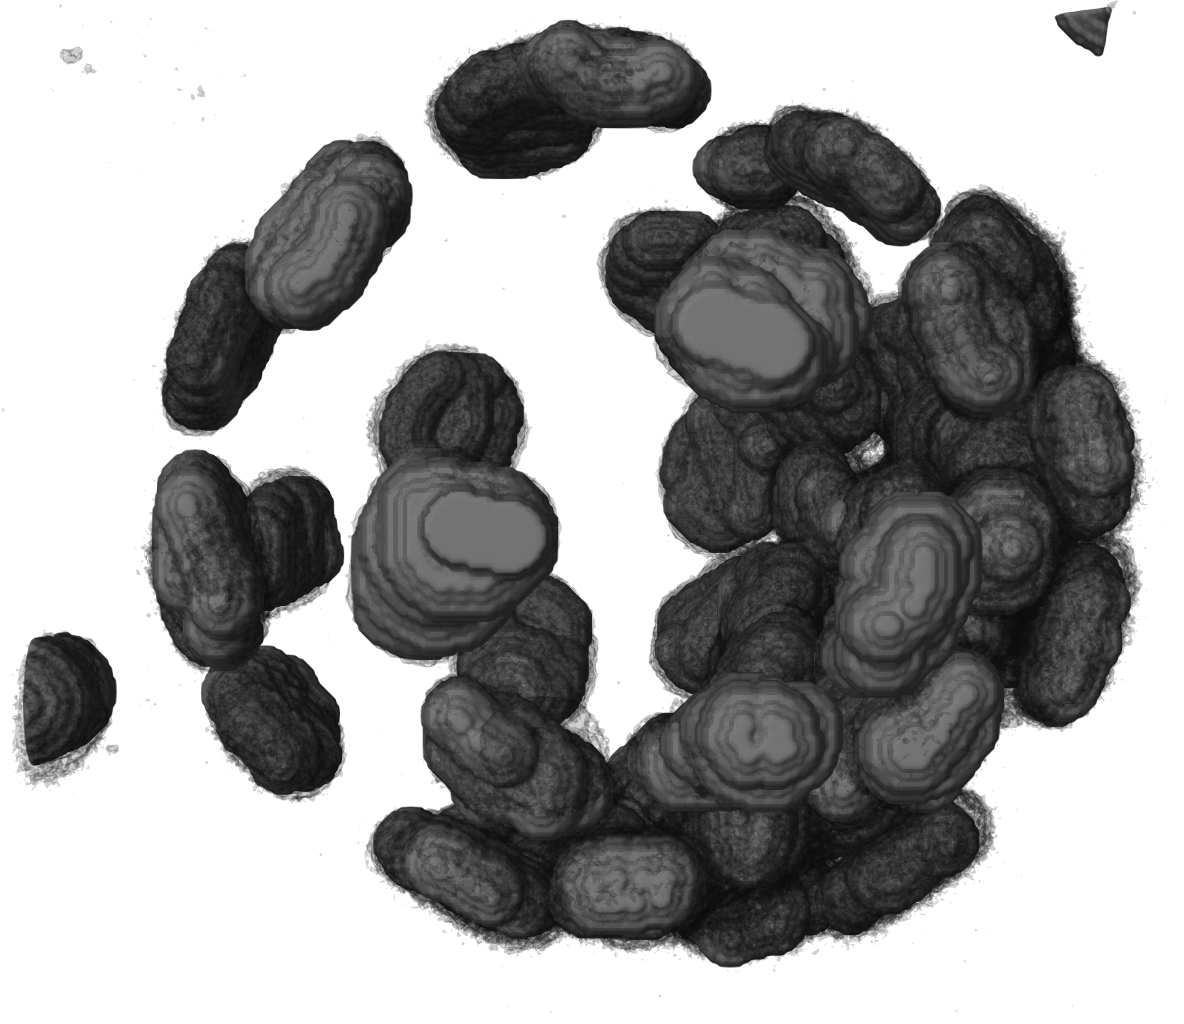
\includegraphics[width=\textwidth]{images/idr-6001240-cvsx.png}
        \caption{Legacy CVSX rendering.}
        \label{fig:idr-6001240-cvsx}
    \end{subfigure}
    \hfill
    \begin{subfigure}{0.45\textwidth}
        \centering
        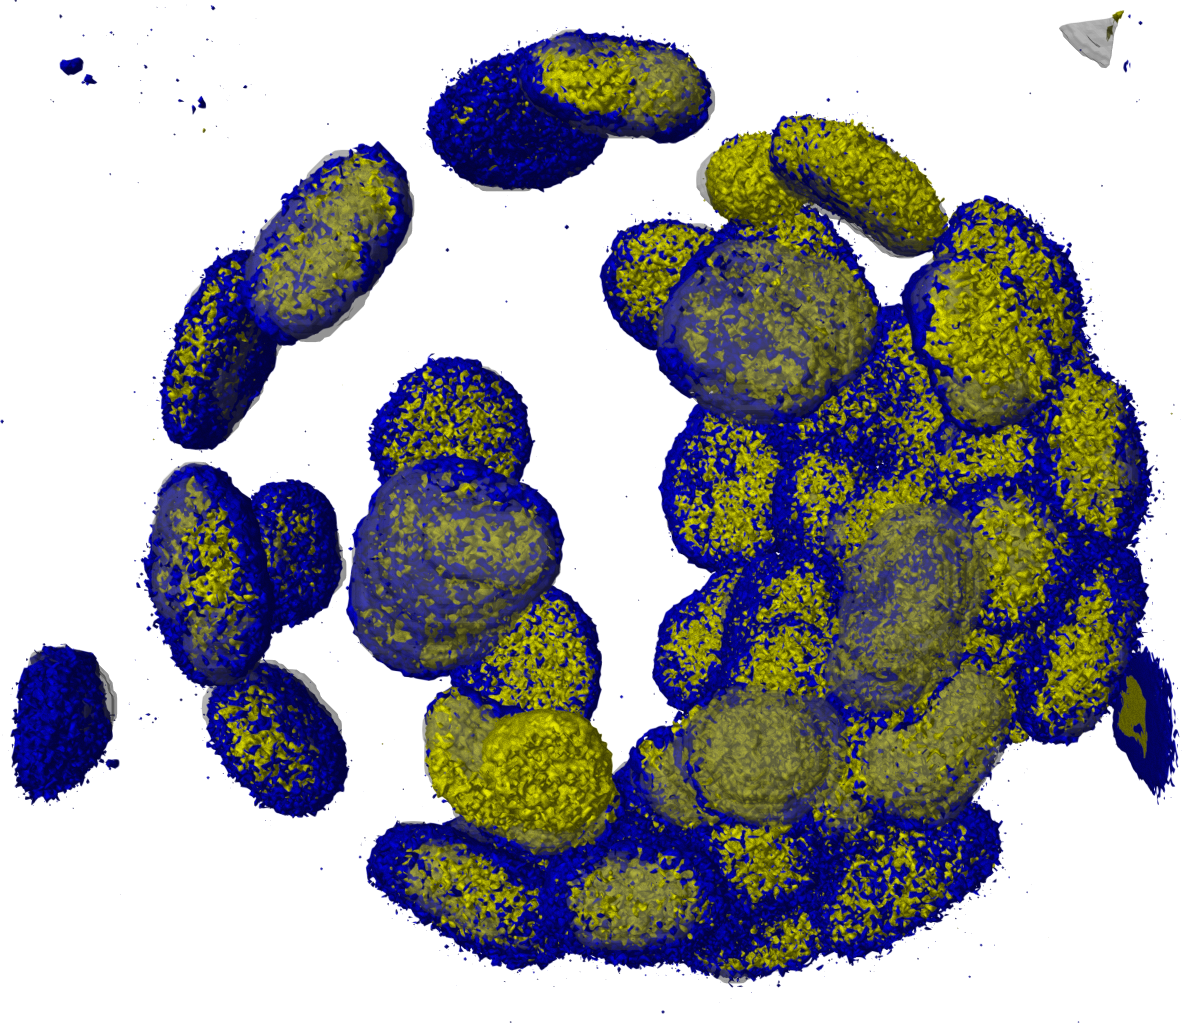
\includegraphics[width=\textwidth]{images/idr-6001240-mvsx.png}
        \caption{MVSX rendering.}
        \label{fig:idr-6001240-mvsx}
    \end{subfigure}
    \caption[Correction of missing annotations]{Correction of missing color annotations for dataset IDR-6001240.}
    \label{fig:visual-comparison}
\end{figure}

\subsubsection{Missing Contours}

The legacy client sometimes fails to fetch the author-defined contour levels from EMDB metadata, despite their being available, which causes the volume to render incorrectly, as shown in Figure~\ref{fig:contour}. As described in Section~\ref{section:fetching-isovalues}, our implementation explicitly fetches this metadata, ensuring the volume is rendered at the correct isovalue.

\begin{figure}[htbp]
    \centering
    \begin{subfigure}{0.45\textwidth}
        \centering
        
\includegraphics[width=\textwidth]{images/contour-missing.png}
        \caption{Legacy CVSX rendering.}
        \label{fig:contour-missing}
    \end{subfigure}
    \hfill
    \begin{subfigure}{0.45\textwidth}
        \centering
        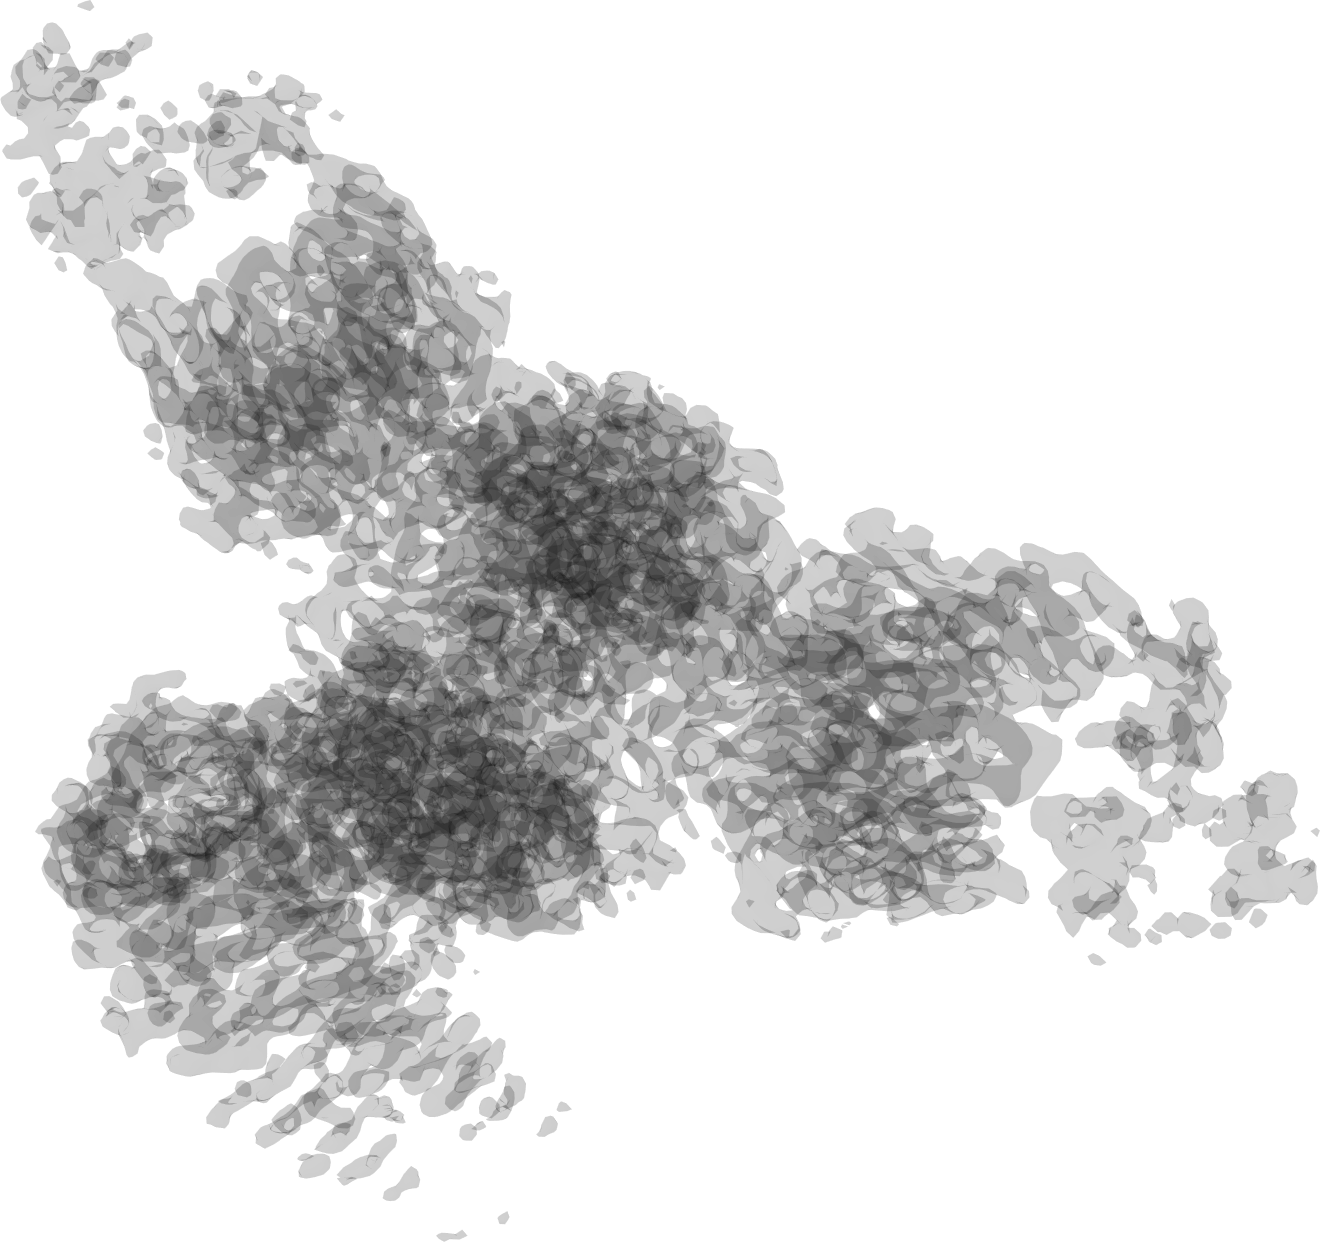
\includegraphics[width=\textwidth]{images/contour-present.png}
        \caption{MVSX rendering.}
        \label{fig:contour-present}
    \end{subfigure}
    \caption[Correction of missing contour level]{Correction of missing author-defined contour levels for dataset EMPIAR-19111.}
    \label{fig:contour}
\end{figure}

\subsubsection{Isosurface Capping}

Lattice isosurfaces that touch the grid boundary were previously rendered as non-watertight meshes with missing faces, as shown in Figure~\ref{fig:missing-face}. As described in Section~\ref{section:impl-lattice}, our implementation pads the lattice voxel grid, which ensures that the generated mesh is closed.

\begin{figure}[htbp]
    \centering
    \begin{subfigure}{0.45\textwidth}
        \centering
        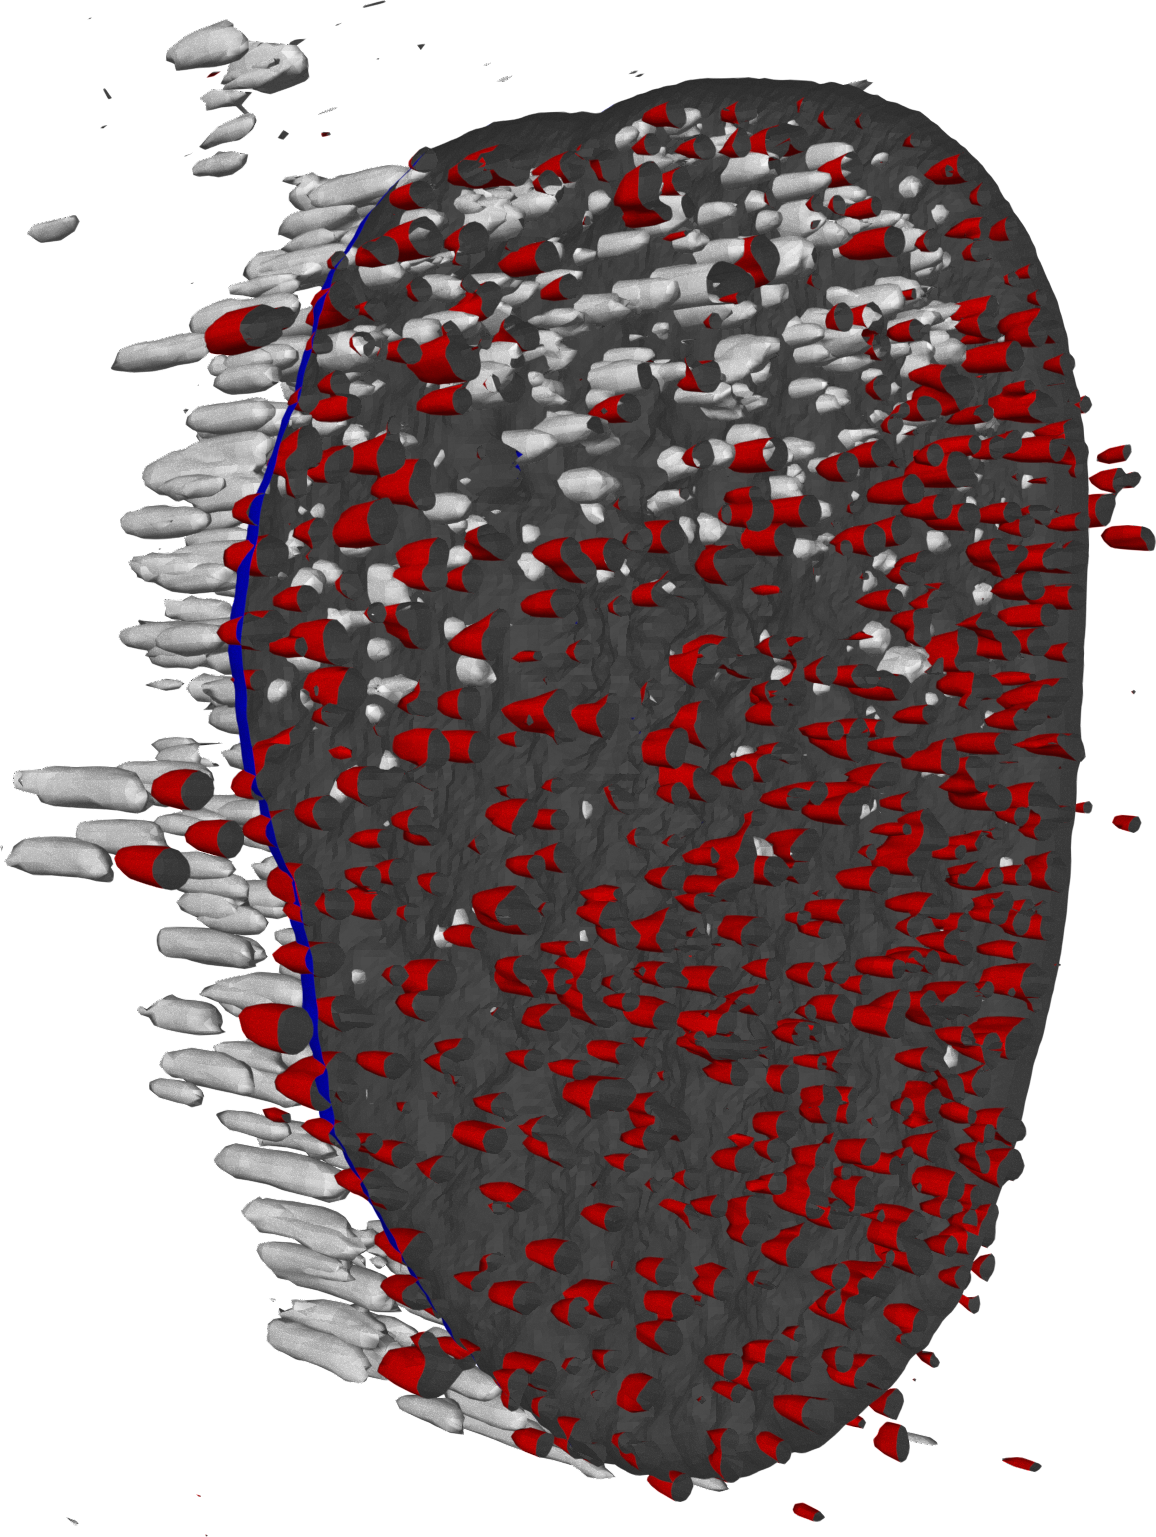
\includegraphics[width=\textwidth]{images/missing-face-cvsx.png}
        \caption{Legacy CVSX rendering.}
        \label{fig:missing-face-cvsx}
    \end{subfigure}
    \hfill
    \begin{subfigure}{0.45\textwidth}
        \centering
        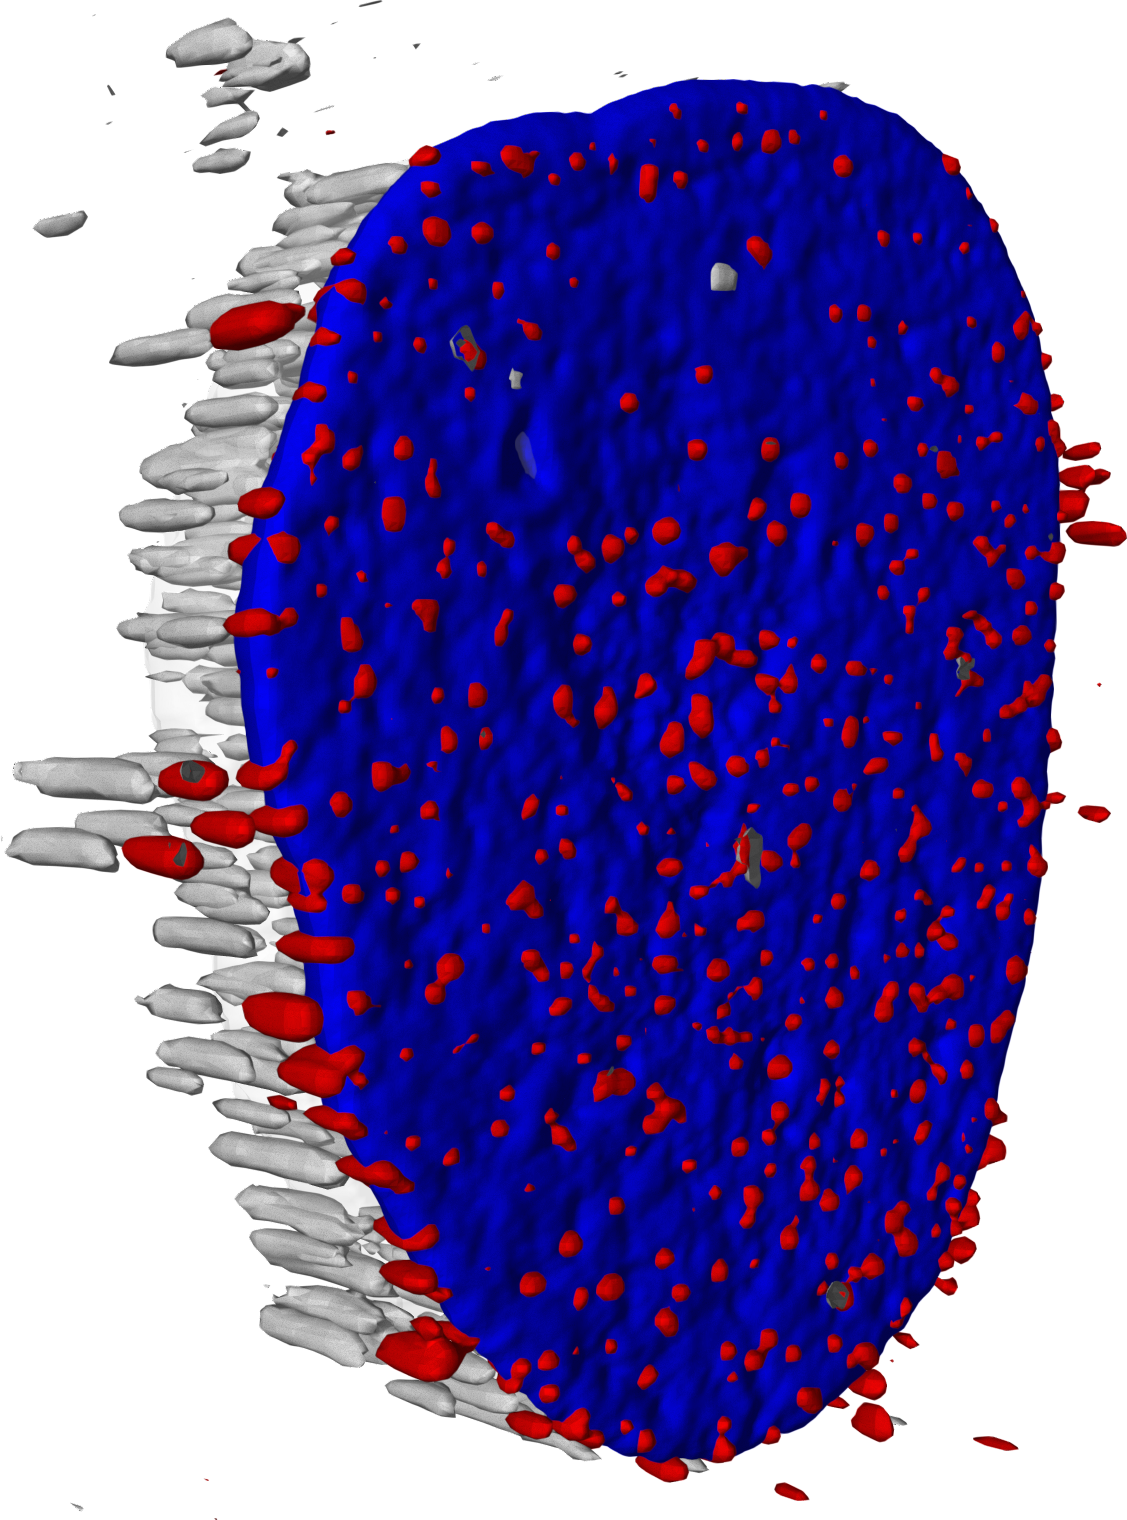
\includegraphics[width=\textwidth]{images/missing-face-mvsx.png}
        \caption{MVSX rendering.}
        \label{fig:missing-face-mvsx}
    \end{subfigure}
    \caption[Correction of isosurface capping]{Correction of isosurface capping for dataset IDR-13457537.}
    \label{fig:missing-face}
\end{figure}

\subsection{Rendering Deviations}

We observed a minor visual discrepancy in the rendering of grid slices (e.g., IDR-5025551). While the data is identical, the converted MVSX visualization appears slightly darker than the original CVSX, as shown in Figure~\ref{fig:slices-comparison}.

Since the conversion library does not modify the raw density values or the opacity parameters for slices, we hypothesize this is caused by updates to the shader or rendering pipeline in the core Mol* Viewer between the version used by the legacy client and the current version. This change affects the visual aesthetics but does not impact the scientific accuracy of the data.

\begin{figure}[htbp]
    \centering
    \begin{subfigure}{0.45\textwidth}
        \centering
        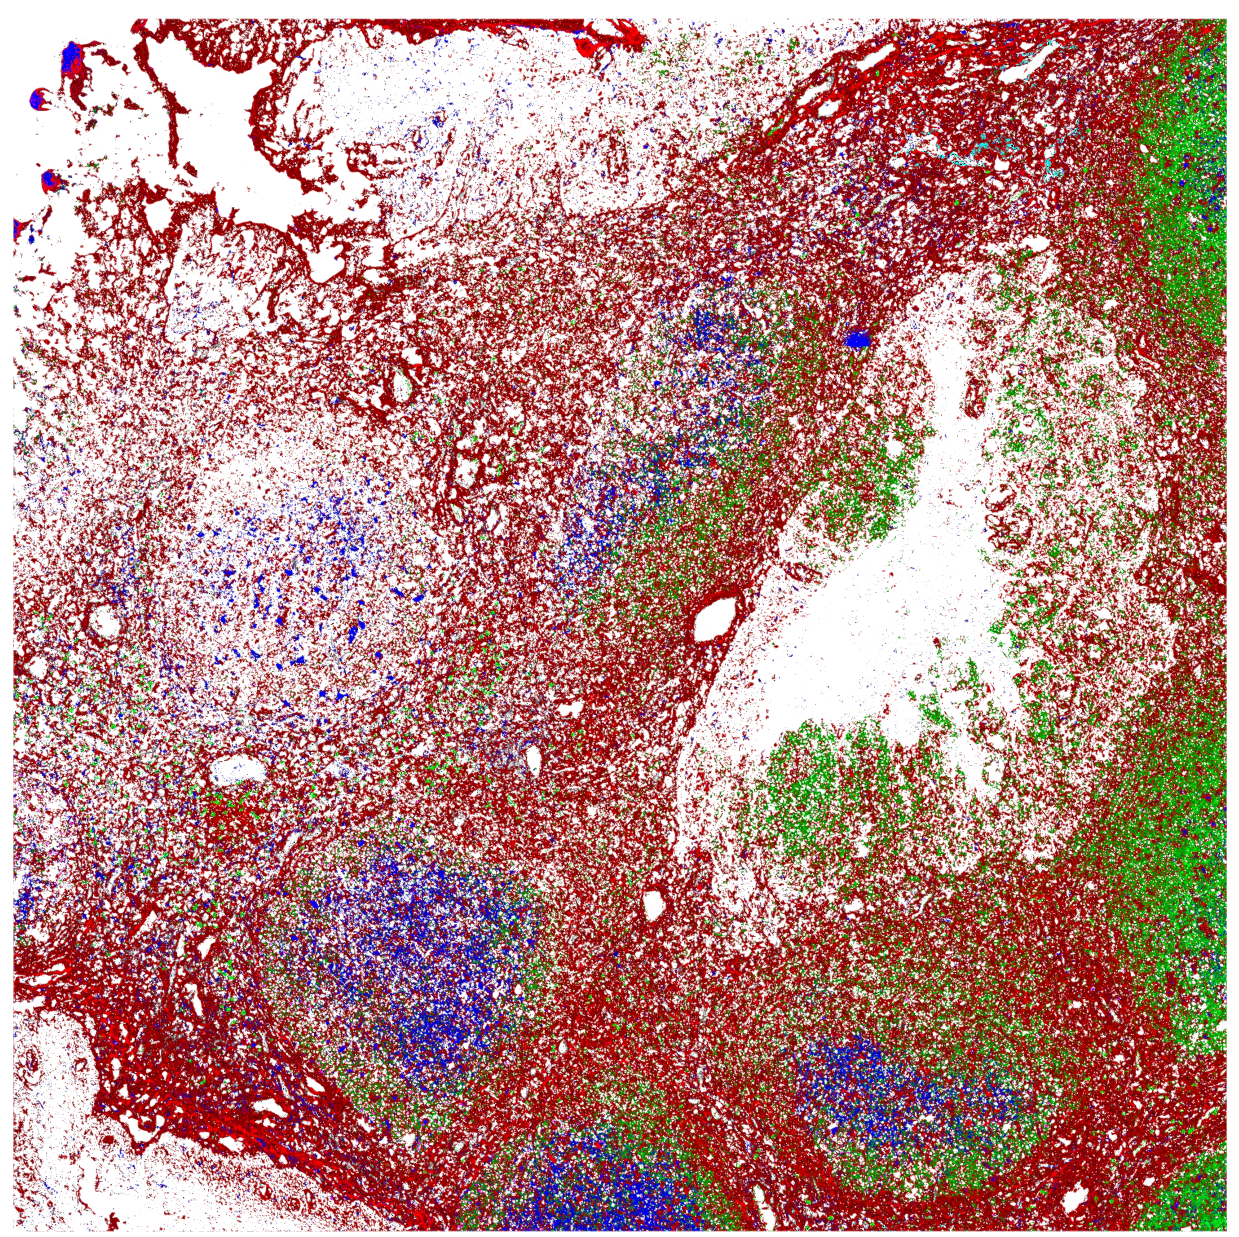
\includegraphics[width=\textwidth]{images/cvsx-slice.png}
        \caption{Legacy CVSX rendering.}
        \label{fig:cvsx-slice}
    \end{subfigure}
    \hfill
    \begin{subfigure}{0.45\textwidth}
        \centering
        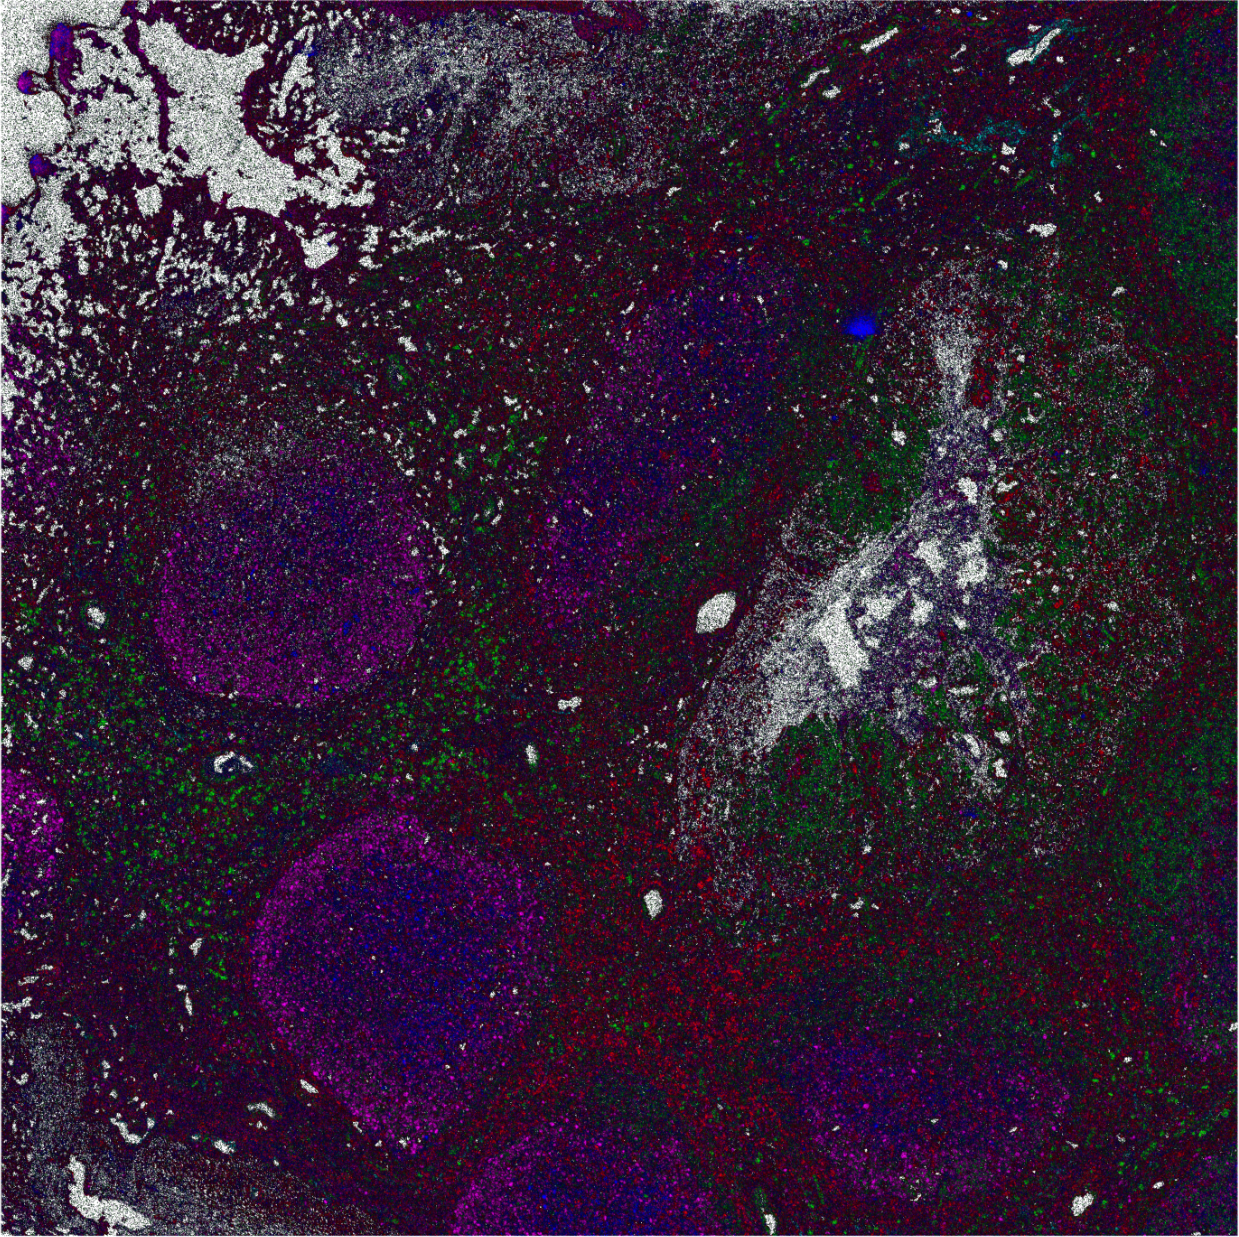
\includegraphics[width=\textwidth]{images/mvsx-slice.png}
        \caption{MVSX rendering.}
        \label{fig:mvsx-slice}
    \end{subfigure}
    \caption[Rendering deviation]{Rendering deviation for dataset IDR-5025551.}
    \label{fig:slices-comparison}
\end{figure}

\subsection{Performance Improvements}

A significant improvement was observed in the handling of geometric segmentations. The legacy client rendered geometric primitives (such as spheres representing ribosomes) individually. For large datasets, such as EMPIAR-11756, which contain hundreds of segments, this approach proved highly inefficient, resulting in prolonged load times and sometimes browser crashes.

The conversion library utilizes the MVS primitives node, which batches these shapes into a single load operation. This approach reduces load times to a fraction of the legacy solution and eliminates browser instability.

\subsection{File Size Analysis}
\label{section:file-size-analysis}

We compared the file sizes of the generated MVSX archives with those of the original CVSX archives.

The results are summarized in Table~\ref{tab:size-comparison}, where the column ``Type'' indicates the nature of the data and the specific conversion strategy employed:

\begin{itemize}
    \item \textbf{Lattice-mesh:} Refers to lattice segmentations (voxel masks) that were converted into surface meshes using the Marching Cubes algorithm.
    \item \textbf{Lattice-volume:} Refers to lattice segmentations that were preserved as volumetric binary masks.
    \item \textbf{Mesh:} Refers to data that was already in mesh format in the source CVSX.
    \item \textbf{Geometric:} Refers to shape primitives (spheres, cylinders, etc.).
    \item \textbf{Volume-only:} Refers to datasets containing only density maps without any segmentation.
\end{itemize}

The analysis reveals that for the majority of data types, the conversion process has a minimal impact on file size. Entries classified as ``mesh'', ``geometric'', and ``volume-only'' typically show deviations of less than 4\%. This indicates that the overhead introduced by the MVSJ tree structure and the MVSX container format is minimal compared to the size of the legacy CVSX format.

However, a significant increase in file size is observed in the ``lattice-mesh'' category, where sizes increased by 11\% to nearly 78\%. This expansion is inherent to the change in data representation. The source CVSX files store this data as voxel masks (RLE compressed), which are highly efficient for solid regions. The converted MVSX files, however, store this data as geometric meshes. For complex biological structures, the explicit definition of thousands of triangular faces requires significantly more storage space. The extreme outlier (EMD-1832, +77.43\%) represents a tiny dataset (0.09 MB); here, the relative increase is magnified by the fixed overhead of the MVSX file structure, although the absolute difference (0.07 MB) is negligible.

Conversely, when the ``lattice-volume'' strategy is employed (preserving the data as voxel masks) the file size increase drops significantly (generally 1--3\%, with the small EMD-1832 outlier at roughly 10\%). This demonstrates that the MVSX format is capable of storing volumetric segmentation as efficiently as the legacy format, provided the appropriate representation is selected.

\begin{table}[ht]
\centering
\caption[Comparison of file sizes]{Comparison of file sizes between original CVSX and converted MVSX formats.}
\label{tab:size-comparison}
\resizebox{\textwidth}{!}{
\begin{tabular}{llrrrr}
\toprule
\textbf{Dataset} & \textbf{Type} & \textbf{CVSX (MB)} & \textbf{MVSX (MB)} & \textbf{Diff (MB)} & \textbf{\% Diff} \\
\midrule
EMD-1832  & lattice-mesh & 0.09 & 0.15 & 0.07 & 77.43\% \\
IDR-13457537 & lattice-mesh & 28.03 & 40.01 & 11.98 & 42.74\% \\
EMD-1273 & lattice-mesh & 39.78 & 47.06 & 7.28 & 18.30\% \\
IDR-6001240 & lattice-mesh & 40.66 & 45.55 & 4.90 & 12.04\% \\
IDR-6001247 & lattice-mesh & 35.43 & 39.48 & 4.05 & 11.42\% \\
\midrule
EMD-1832 & lattice-volume & 0.09 & 0.09 & 0.01 & 9.89\% \\
IDR-6001240 & lattice-volume & 40.66 & 42.09 & 1.43 & 3.52\% \\
IDR-6001247 & lattice-volume & 35.43 & 36.37 & 0.94 & 2.65\% \\
EMD-1273 & lattice-volume & 39.78 & 40.23 & 0.45 & 1.14\% \\
IDR-13457537 & lattice-volume & 28.03 & 28.28 & 0.25 & 0.91\% \\
\midrule
EMPIAR-10070  & mesh         & 56.30 & 56.72 & 0.42 & 0.75\% \\
\midrule
EMPIAR-11756  & geometric    & 3.93 & 3.86 & -0.08 & -1.98\% \\
\midrule
IDR-5514375 & volume-only & 493.08 & 509.48 & 16.40 & 3.33\% \\
IDR-5025553 & volume-only & 96.63 & 96.77 & 0.15 & 0.15\% \\
IDR-5025552 & volume-only & 63.29 & 63.37 & 0.08 & 0.12\% \\
IDR-5025551 & volume-only & 65.92 & 66.00 & 0.08 & 0.12\% \\
CUSTOM-19420 & volume-only & 32.22 & 32.22 & 0.00 & 0.00\% \\
CUSTOM-TUBHISWT & volume-only & 106.10 & 106.09 & 0.00 & 0.00\% \\
EMD-19111 & volume-only & 12.15 & 12.15 & 0.00 & 0.00\% \\
\bottomrule
\end{tabular}
}
\end{table}

\clearpage
\newpage
\chapter{Web Application}
\label{chapter:app}

While the conversion library described in Chapter~\ref{chapter:library} provides the computational engine for data transformation, it remains a command-line tool accessible primarily to users with programming expertise. However, the target demographic for this tool---structural biologists and educators---typically requires a graphical interface to interact with data intuitively. 

Beyond simply providing access to the conversion process, there is also a need to improve the workflow for editing the datasets' annotations. The legacy Mol* VS tool offered some basic annotation capabilities, although editing these annotations required manual modification of JSON files, a process that was unintuitive and prone to syntax errors.

To address these usability gaps, we developed a full-stack web application. This application democratizes access to the conversion pipeline, introduces a ``What You See Is What You Get'' (WYSIWYG) editor for biological annotations, and provides a persistent storage solution for sharing visualizations.

Section~\ref{requirements} covers the requirements of this web application, followed by Section~\ref{section:app-design}, which covers the design and architecture of the application. Finally, Section~\ref{section:app-implementation} describes the implementation and deployment.

\section{Requirements}
\label{requirements}

The following sections outline the requirements for implementing the web application, categorizing them into functional and non-functional categories.

\subsection{Functional Requirements} 
\label{functional-requirements}

Functional requirements describe how the system should behave. The key functional areas of the application are defined as follows:

\subsubsection{Entry Management}
\label{section:entry-management-requirement}

The system must allow authenticated users to manage their converted entries (i.e., converted CVSX datasets). Managing the entries requires the ability to create new entries by uploading the legacy CVSX archive files and running the conversion process. Crucially, the upload process must enforce storage quotas to prevent resource exhaustion. Furthermore, users must be able to list their converted entries, update the entry's metadata, and delete the entries they no longer need.

\subsubsection{Viewer and Annotation Editor}
\label{section:annotation-editor-requirement}

The system must allow users to modify the annotations of their entries interactively, including adjusting the visual (e.g., opacity, isovalue) and textual (e.g., names, descriptions) annotations of the entries. These changes must be persisted to the backend storage and synchronized on the frontend with the Mol* Viewer to provide visual feedback.

\subsubsection{Sharing and Export}
\label{section:sharing-requirement}

To support collaboration, the system must allow users to share their entries via a persistent URL share link. These share links allow unauthenticated users (guests) to view specific entries without requiring a login. 

Additionally, the system acts as a bridge to the broader Mol* ecosystem. While the internal viewer provides essential inspection tools, it is not designed for complex scene composition (e.g., superimposing atomic models from the PDB or creating cinematic camera transitions). To address this, the system allows users to export their entries as MVStory archives or open them directly in the external MolViewStories application. 

This feature is critical for the ``scientific storytelling'' workflow: our application handles the challenging task of converting and hosting the raw volumetric data, providing the user with a pre-configured ``base story''. The user can then transfer this story to the external MolViewStories builder to layer on rich biological context---such as fetching related protein structures, adding educational labels, or refining visual styling---capabilities that go beyond the scope of the simple internal viewer.

\subsubsection{API Access}
\label{section:api-access}

All functionality available in the web interface---uploading, editing, and sharing---must be exposed via a public RESTful application programming interface (API). This API must be integrable into third-party workflows or automated scripts.

\subsection{Non-Functional Requirements}
\label{section:non-functional-requirements}

Several non-functional requirements constrain the system architecture. These constraints dictate the specific technologies and architectural patterns used throughout the implementation:

\subsubsection{Security and Authentication}
\label{section:security-requirements}

Access to the web user interface must be protected using the OpenID Connect (OIDC)\footnote{\url{https://openid.net}} protocol, specifically configured to integrate with the EINFRA AAI\footnote{\url{https://aai.cesnet.cz}} infrastructure. This approach eliminates the risks associated with storing user credentials internally and provides a seamless single sign-on (SSO) experience for researchers across different institutions supported by EINFRA AAI.

\subsubsection{Infrastructure and Deployment}
\label{section:deployment-requirement}

For production deployment, all system components must be containerized using Docker\footnote{\url{https://www.docker.com}}, and the system deployment is required to run on a Kubernetes\footnote{\url{https://kubernetes.io}} cluster, specifically utilizing the CERIT-SC Kubernetes Container Platform\footnote{\url{https://docs.cerit.io/en/docs/platform/overview}}. The deployment process manages the entire deployment configuration using Helm\footnote{\url{https://helm.sh}}. Furthermore, the production deployment must be automated via a continuous integration and continuous delivery (CI/CD) pipeline.

\subsubsection{Data Storage}
\label{section:data-requirement}

The system requires a two-type storage solution to handle the distinct nature of the data. The system must store entry metadata, share links, and user profiles in a relational database. It must offload large binary files, such as the volumetric and segmentation files extracted from the CVSX archives, to an object storage solution.

\subsubsection{Performance}
\label{section:perf-requirement}

The system must remain responsive during resource-intensive operations, such as during the CVSX file conversion.

\subsubsection{Documentation}
\label{section:doc-requirement}

The system implementation requires comprehensive documentation that describes the codebase structure, API specification, and deployment procedures to ensure the system's maintainability and long-term viability.

\section{Design} 
\label{section:app-design}

The system is architected as a modern, decoupled web application designed to separate data processing responsibilities from user interaction. The core of the system relies on a client-server model where a RESTful API gateway orchestrates the communication between the user interface and the underlying data services.

\subsection{System Architecture}
\label{section:system-arch}

The application logic is distributed across four primary services, each running in its own container to ensure separation of concerns, isolation, and scalability. The Figure~\ref{fig:arch} highlights this architecture.

\begin{figure}[htbp]
    \centering
    \includegraphics[width=0.5\textwidth]{images/system-architecture.pdf}
    \caption[Web application system architecture]{Container diagram showing the interactions between the web, API, and storage services.}
    \label{fig:arch}
\end{figure}

\subsubsection{Web Service}
\label{section:web-service}

The frontend web service acts as the presentation layer and is a single-page application (SPA) served via Nginx\footnote{\url{https://nginx.org}}. It is responsible for the interactive elements of the application, including the Mol* 3D viewer and the annotation editor form. 

The SPA communicates exclusively with the API service via HTTP requests, which are protected with JWT cookie authentication derived from the OIDC provider access tokens.

\subsubsection{API Service}
\label{section:api-service}

The backend API service serves as the central gateway for all requests. It handles authentication and authorization, request validation, and business logic. 

Crucially, the service is fully asynchronous and schedules heavy processing jobs to run in separate threads. This approach ensures that heavy conversion jobs do not block the web server's main thread, allowing it to remain responsive and efficient.

The API implements a dual-authentication strategy. While the SPA utilizes JWT cookies for authentication, third-party scripts and external workflows authenticate via API keys. These keys are opaque tokens generated by the user.

\subsubsection{Data Persistence}
\label{section:data-services}

Two specialized storage solutions handle the data persistence. PostgreSQL\footnote{\url{https://www.postgresql.org}} is used for the relational database, while MinIO\footnote{\url{https://www.min.io}} serves as the object storage solution and stores the unstructured binary data.

\subsection{Database Design}
\label{section:database-design}

The entity-relationship diagram in Figure~\ref{fig:er-diagram} captures the database schema. The core entity is the \texttt{User}, which stores identity information linked to the external OIDC provider.

The central data entity is the \texttt{Entry}, which represents a single uploaded and converted CVSX file. The schema tracks the lifecycle of an entry through a status enumeration---Pending, Processing, Completed, and Failed.

Sharing entries is implemented through the \texttt{ShareLink} entity. This entity maintains a one-to-one relationship with an entry. It creates a decoupling layer that allows an entry to be accessed via a unique UUID token rather than the Entry's internal database ID, allowing the user to turn off the share link if needed.

Finally, the \texttt{ApiKey} entity represents API keys generated by the user. To ensure security, instead of storing the API key directly, the database stores a cryptographic hash of the key; the raw key is never stored in the database, meaning it is displayed to the user only once upon creation.

\begin{figure}[htbp]
    \centering
    \includegraphics[width=0.8\textwidth]{images/er-diagram.pdf}
    \caption[Entity-relationship diagram]{Entity-relationship diagram describing the design of the database.}
    \label{fig:er-diagram}
\end{figure}

\section{Implementation}
\label{section:app-implementation}

This section details the implementation of the core system components. It covers the use of existing technologies, implementation of the web user interface, and deployment of the system.

\subsection{Used Technologies}

The application is built using a modern decoupled architecture, consisting of a TypeScript-based single-page application for the frontend and a Python-based REST API for the backend.

\subsubsection{Frontend}

The frontend SPA is developed using the React library. React's component\allowbreak-based architecture promotes code reusability and allows for the seamless integration of the Mol* Viewer as a distinct DOM element.

To ensure a robust and accessible user interface and handle synchronization with the server state, the application leverages several key libraries:

\begin{itemize}
    \item \textbf{ShadCN\footnote{\url{https://ui.shadcn.com}}:} A UI component library built on top of RadixUI.
    
    \item \textbf{Tailwind CSS\footnote{\url{https://tailwindcss.com}}:} A utility-first CSS framework used for styling.
    
    \item \textbf{TanStack Query\footnote{\url{https://tanstack.com/query}}:} An asynchronous state management library that is used to synchronize server state on the client side.
    
    \item \textbf{HeyAPI Code Generator\footnote{\url{https://heyapi.dev}}:} To ensure strict type safety between the frontend and backend, the API client SDK is automatically generated from the OpenAPI specification of the API service. This ensures that any changes in the API schema are immediately reflected in the frontend code, preventing runtime errors caused by interface mismatches.
\end{itemize}

\subsubsection{Backend}

The backend API service is implemented in Python, ensuring consistency with the conversion library described in Chapter~\ref{chapter:library}. The core framework chosen is FastAPI, which was selected for several reasons:

\begin{itemize}
    \item \textbf{Asynchronous Support:} It offers native support for Python's asyncio\footnote{\url{https://docs.python.org/3/library/asyncio.html}} capabilities, which is critical for handling concurrent requests while managing long-running I/O operations, such as file uploads to object storage.
    
    \item \textbf{Data Validation:} It is tightly integrated with Pydantic\footnote{\url{https://pypi.org/project/pydantic}}, which provides data validation and settings management using Python type annotations. This ensures that all incoming requests adhere to the defined schema before processing.
    
    \item \textbf{Automatic Documentation:} FastAPI automatically generates interactive API documentation (Swagger UI\footnote{\url{https://swagger.io/tools/swagger-ui}}), which facilitates testing and integration for third-party developers.
\end{itemize}

For data persistence and management, the backend utilizes:

\begin{itemize}
    \item \textbf{SQLAlchemy\footnote{\url{https://pypi.org/project/SQLAlchemy}}:} An Object Relational Mapper (ORM) that serves as the abstraction layer for the PostgreSQL database. It enables the manipulation of database entries using Python objects rather than raw SQL, thereby improving code readability and security. Furthermore, the SQLAlchemy ORM is configured with asyncpg\footnote{\url{https://pypi.org/project/asyncpg}}, which enables asynchronous communication with the database.
    
    \item \textbf{Alembic\footnote{\url{https://pypi.org/project/alembic}}:} A lightweight database migration tool used in conjunction with SQLAlchemy. It manages schema changes (version control) over time, ensuring that the database structure remains consistent across development, testing, and production environments.
    
    \item \textbf{MinIO Client\footnote{\url{https://pypi.org/project/minio}}:} The official Python client for interacting with the MinIO object storage. It handles streaming of large binary files (CVSX archives) to and from the storage buckets.
\end{itemize}

\subsection{Application Workflow}

The application workflow is divided into two distinct functional areas: the entries dashboard for data management and the annotation editor for viewing and updating the annotations of entries.

\subsection{Entries Dashboard}

The primary entry point of the application is the entries dashboard view, shown in Figure~\ref{figure:dashboard-page}. This view contains a list of users' entries. The user can preview these entries, download them in MVSX or MVStory formats, export them to the external MolViewStories application, or share them with others via a share link.

The interface is designed to handle the asynchronous nature of the conversion pipeline effectively. When a user uploads a legacy CVSX archive, the entry is immediately added to the list with a ``Processing'' status indicator. This status updates in real-time (via polling or invalidation strategies), allowing the user to continue working or navigate away without interrupting the server-side conversion.

The dashboard also displays storage quota usage, providing users with immediate visibility into their resource consumption.

\begin{figure}[htbp]
    \centering
    \includegraphics[width=0.8\textwidth]{images/dashboard.png}
    \caption[Entries dashboard view]{View of the entries dashboard page, which allows managing the user's entries and exporting them.}
    \label{figure:dashboard-page}
\end{figure}

\subsection{Annotation Editor}

Unlike the legacy Mol* VS Client implementation, which essentially required manual JSON editing of the annotations, this editor provides a GUI-based approach for editing them. The annotations editor, displayed in Figure~\ref{fig:app-editor}, allows editing both the visual (e.g., opacity, isovalue) and descriptive (e.g., descriptions, tooltips) annotations of the user's volume and segmentation data. These updates are persisted to the backend, unlike modifications in the legacy Mol* VS Client, which were persisted only for the current browser session.

The visualization of the updated entry is handled by the Mol* Viewer.

\begin{figure}[htbp]
    \centering
    \includegraphics[width=0.8\textwidth]{images/preview page.png}
    \caption[Annotation editor view]{View of the annotations editor. On the left side of the page is a list of volumes and segmentations which the user can edit, while on the right side of the page is the preview of the entry in Mol* Viewer.}
    \label{fig:app-editor}
\end{figure}

\subsection{Deployment and Infrastructure}
\label{section:deployment}

The system is containerized via Docker and deployed to a Kubernetes production environment via Helm and a CI/CD pipeline. This approach isolates dependencies, preventing configuration drift and simplifying the scaling of individual services.

\subsubsection{Containerization}

Both the web service and the API service are defined using a Dockerfile and built into container images with Docker. For local development, the orchestration of these containers — along with the database and object storage services — is managed via Docker Compose\footnote{\url{https://docs.docker.com/compose}}, mirroring the Kubernetes production deployment, albeit on a single machine.

\subsubsection{Kubernetes Orchestration}

For production, the system is deployed on the ``kuba'' cluster, a Kubernetes cluster provided by the CERIT-SC Kubernetes Container Platform. Kubernetes was chosen for its ability to handle automatic scaling, self-healing (restarting failed containers), and declarative configuration management. 

The configuration of the Kubernetes deployment is captured in Figure~\ref{figure:k8s}. It is managed using Helm charts that define the following Kubernetes resources:

\begin{itemize}
    \item \textbf{Deployments:} Define the stateless application services (web, API, MinIO) with resource limits.
    
    \item \textbf{Config Maps and Secrets:} Define the environment variables and secrets used by the Pods of the corresponding Deployments.
        
    \item \textbf{Persistent Volume Claims (PVCs):} Request durable storage from the underlying infrastructure to ensure that database records and object files survive pod restarts or node migrations.
    
    \item \textbf{Ingress:} External access to the web and API services is handled through Nginx ingress controllers.
\end{itemize}

\subsubsection{CI/CD Pipeline}

The release process is fully automated using a CI/CD pipeline implemented in GitHub Actions\footnote{\url{https://docs.github.com/en/actions}}. This pipeline is triggered on every push to the main branch of the GitHub repository and executes the following workflow:

\begin{enumerate}    
    \item \textbf{Build and Registry Push:} The pipeline checks out the source code, builds the Docker images for the web and API services, and pushes the built images to the Harbor\footnote{\url{https://hub.cerit.io}} image registry.
    
    \item \textbf{Deployment:} The pipeline authenticates with the Kubernetes cluster and executes a Helm upgrade command, which updates the cluster configuration to use the newly pushed images, triggering a rolling update of the application with zero downtime.
\end{enumerate}

\begin{figure}[htbp]
    \centering
    \includegraphics[width=0.9\textwidth]{images/k8s-deployment2.pdf}
    \caption[Kubernetes deployment configuration]{Kubernetes deployment configuration for the web application containers.}
    \label{figure:k8s}
\end{figure}

\subsection{Availability}

Both the implemented web service and the API service are available online via the following URL links:

\begin{itemize}
  \item \textbf{Web service:} \\
  \url{https://web.volseg-editor.dyn.cloud.e-infra.cz/}
  \item \textbf{API service:} \\
  \url{https://api.volseg-editor.dyn.cloud.e-infra.cz/docs}
\end{itemize}

\clearpage
\bookmarksetup{startatroot}
\addtocontents{toc}{\bigskip}

\chapter*{Conclusion}
\label{chapter:conclusion}
\markright{\textsc{Conclusion}}
\addcontentsline{toc}{chapter}{Conclusion}

The primary objectives of this thesis were to develop a lightweight web application for visualizing and annotating volumetric and segmentation data in Mol* and to bridge the gap between the legacy Mol* VS implementation and the modern Mol* ecosystem. We achieved this through two complementary practical contributions.

Firstly, we developed a conversion library that maps the data types of the legacy CVSX format to the modern MVSX and MVStory formats. As demonstrated in the verification chapter, the library not only preserves visual fidelity but also corrects historical rendering artifacts found in the legacy client.

Secondly, we developed a web application that provides access to these conversion tools through an intuitive user interface and an API, and also serves as a lightweight annotation editor for annotating the converted volume and segmentation data. For more advanced annotations, the application allows exporting the data into the modern MolViewStories application to facilitate further annotation.

Finally, the data processing logic and mapping definitions developed in this thesis will serve as a foundation for the design of the new Mol* VS preprocessor, directly influencing how volumetric data will be packaged in future versions of the platform.

\printbibliography[heading=bibintoc]

\appendix

\chapter{Attachments}
\label{chapter:source-code}

The source code is attached as a ZIP archive in the submission vault available at \url{https://is.muni.cz/auth/th/z9y0g/}:

\begin{itemize}
  \item \textbf{Conversion library:} cvsx2mvsx.zip
  \item \textbf{Web application:} volseg-editor.zip
\end{itemize}

The source code is also available in the corresponding GitHub repositories:

\begin{itemize}
  \item \textbf{Conversion library:} \\
  \url{https://github.com/dominikandrewtichy/cvsx2mvsx}
  \item \textbf{Web application:} \\
  \url{https://github.com/dominikandrewtichy/volseg-editor}
\end{itemize}

\end{document}